\clearpage
% \ifx \notincludehead\undefined
\normalsize
\end{document}
\fi


\newpage
\subsection{Управление и диспетчеризация производства}
\label{bp:production}

% На производстве работает 16 машинистов, 2 погрузчика (водителя), 1 грузчик, 1 инженер технолог, 1 инженер качества, 1 комплектовщик оснастки, 1 мастер смены.


%Производство работает в четыре смены. Смены обозначают буквами «А», «Б», «В» и «Г».

%На предприятии разработаны планы по производительности на месяц по сменам (рис. \ref{pic:f35}, \ref{pic:f36}).

\textbf{Выработка гофроагрегата}

Бригада гофроагрегата состоит из 7 человек.

Все задания на гофроагрегат отдел планирования производства передает бригадиру в печатном виде (рис. \ref{pic:Задание на ГА}). Задание печатается из системы 1С: УПП. Реализовано несколько печатных форм для более удобного просмотра информации по количеству, рилевкам, сырью. Бригадир на основе информации по остаткам сырья записывает для водителя погрузчика план подачи рулонов. 

На сухой части ввод заданий и контроль по рилевкам, полосам, размерам и количеству заготовок осуществляется машинистом в ручную на пультах управления гофроагрегатом (рис. \ref{pic:V задание на резке}, \ref{pic:V задание рилевки}). Факт записывается по счетчику и заносится машинистом в систему 1С: УПП (рис. \ref{pic:Vвнесениевыработки}). Перевыпуск по заданию возможен в случае брака или необходимости доработать рулон. Машинист на сухой части производит печать бирок на полуфабрикаты и товарный гофрокартон (рис. \ref{pic:V.10}) из системы 1С: УПП. Высота стопы на съеме определяется машинистами самостоятельно, кроме товарного листа, в этом случае информация берется из ТК.
На мокрой части в системе 1С: УПП фиксируются рулоны по каждому раскату отдельно. При этом в первую очередь перерабатываются частично переработанные рулоны.

Машинист фиксирует все простои гофроагрегата в специальном бланке, указывает причину, также в данном бланке ставит подписи дежурный ремонтный персонал. 

Машинисты ведут журнал технологических параметров (рис. \ref{pic:V журнал техн параметров}). 

Машинисты ведут специальный журнал, где фиксируются замечания по работе оборудования.
Бригада гофроагрегата постоянно взаимодействует с отделом управления качеством. Контролеры ОУК берут на анализ образцы с каждого задания и затем сообщают результаты бригадиру. 

Водители погрузчиков забирают поддоны с заготовками и ориентируясь на маршрут, указанный на бирке отвозят заготовки к соответствующим линиям. Но периодически они вынуждены складировать заготовки на любое свободное место в цехе. Наиболее часто данная ситуация возникает, если гофроагрегат дополнительно работал в ночную смену.    
%Бригадир ГА получает На план у мастера смены (если до этой смены на ГА был выходной или это делает предыдущая смена), раскладывает задания по тому порядку, как удобно выпускать на ГА, просчитывает необходимое сырье для начала работы. Сырье на ГА доставляется грузовой машиной со склада (см. процесс ''Списание сырья'' \ref{bp:MatOutput}). 




\textbf{Выработка линии переработки}

Машинист линии переработки получает задание от отдела планирования производства в бумажном виде (рис. \ref{pic:VI задание для переработки}). 
Краску привозит на линию специалист по подготовке производства.
Оснастка находится в стеллажах у каждой линии переработки (рис. \ref{pic:II хранение фпф}).

После завершения работ по настройке оборудования машинист начинает выпуск изделий, не дожидаясь разрешения контролера ОУК, т.к. один контролер не успевает на все линии. Но машинист всегда оставляет образец для контроля (рис. \ref{pic:V образцы для ОТК}). Машинист совместно с контролером ОУК заполняют специальный бланк по контролю качества по каждому заданию (рис. \ref{pic:VI}).   
Машинист фиксирует факт выработки в системе 1С: УПП (рис. \ref{pic:VI рабочее место машиниста}). Машинист печатает в системе 1С: УПП  бирки на готовую продукцию (рис. \ref{pic:III.10}). После того как бирка напечатана, продукция считается перемещенной на склад, хотя физически она может быть не еще не произведена. 
Дополнительно машинисты фиксируют факт выработки в журнале (рис. \ref{pic:VI журнал машинистов}).
Простои оборудования машинист фиксирует на специальном бланке, который заполняет совместно с дежурным персоналом (аналогично ЛГК).
Замечания по работе также фиксируются в специальном журнале.

\textbf{Мастер}

Мастер осуществляет контроль за работой производства используя различные отчеты  в системе 1С: УПП (рис. \ref{pic:III отчеты 2}).
Мастер  осуществляет контроль за работой ручных линий переработки и фиксирует выработку в системе 1С: УПП. Мастер с печатает бирки на готовую продукцию.
Мастер формирует в системе 1С: УПП отчет по выработке по ручным операциям и сдает его в бухгалтерию. 
Мастер формирует в системе 1С: УПП ''Сменно-суточный рапорт'' (рис. \ref{pic:III.6}). 
Мастер заполняет в системе 1С: УПП электронный табель и сдельные наряды (рис. \ref{pic:IIIсдельныйнаряд}).
Дополнительно данные по выработке производства за смену мастера фиксируют в журнале (рис. \ref{pic:IIIжурналмастера}).
%Каждую смену прессовщики передают мастеру бланки с указанием количества тюков макулатуры (рис. \ref{pic:III.3}). Мастер в системе 1С: УПП формирует акт.
Мастер каждую смену печатает графики простоев по каждому рабочему центру.

% Первые коробки принимает ОТК. Контролер ОТК заполняет и ставит подпись в бланке ф.23, который хранится в ОТК. Брак, внесенный в бланк, руками не пересчитывается, т.к. один контролер не успевает на все линии, заполняет по мере возможности. 

\clearpage



\begin{figure}
\begin{center}
 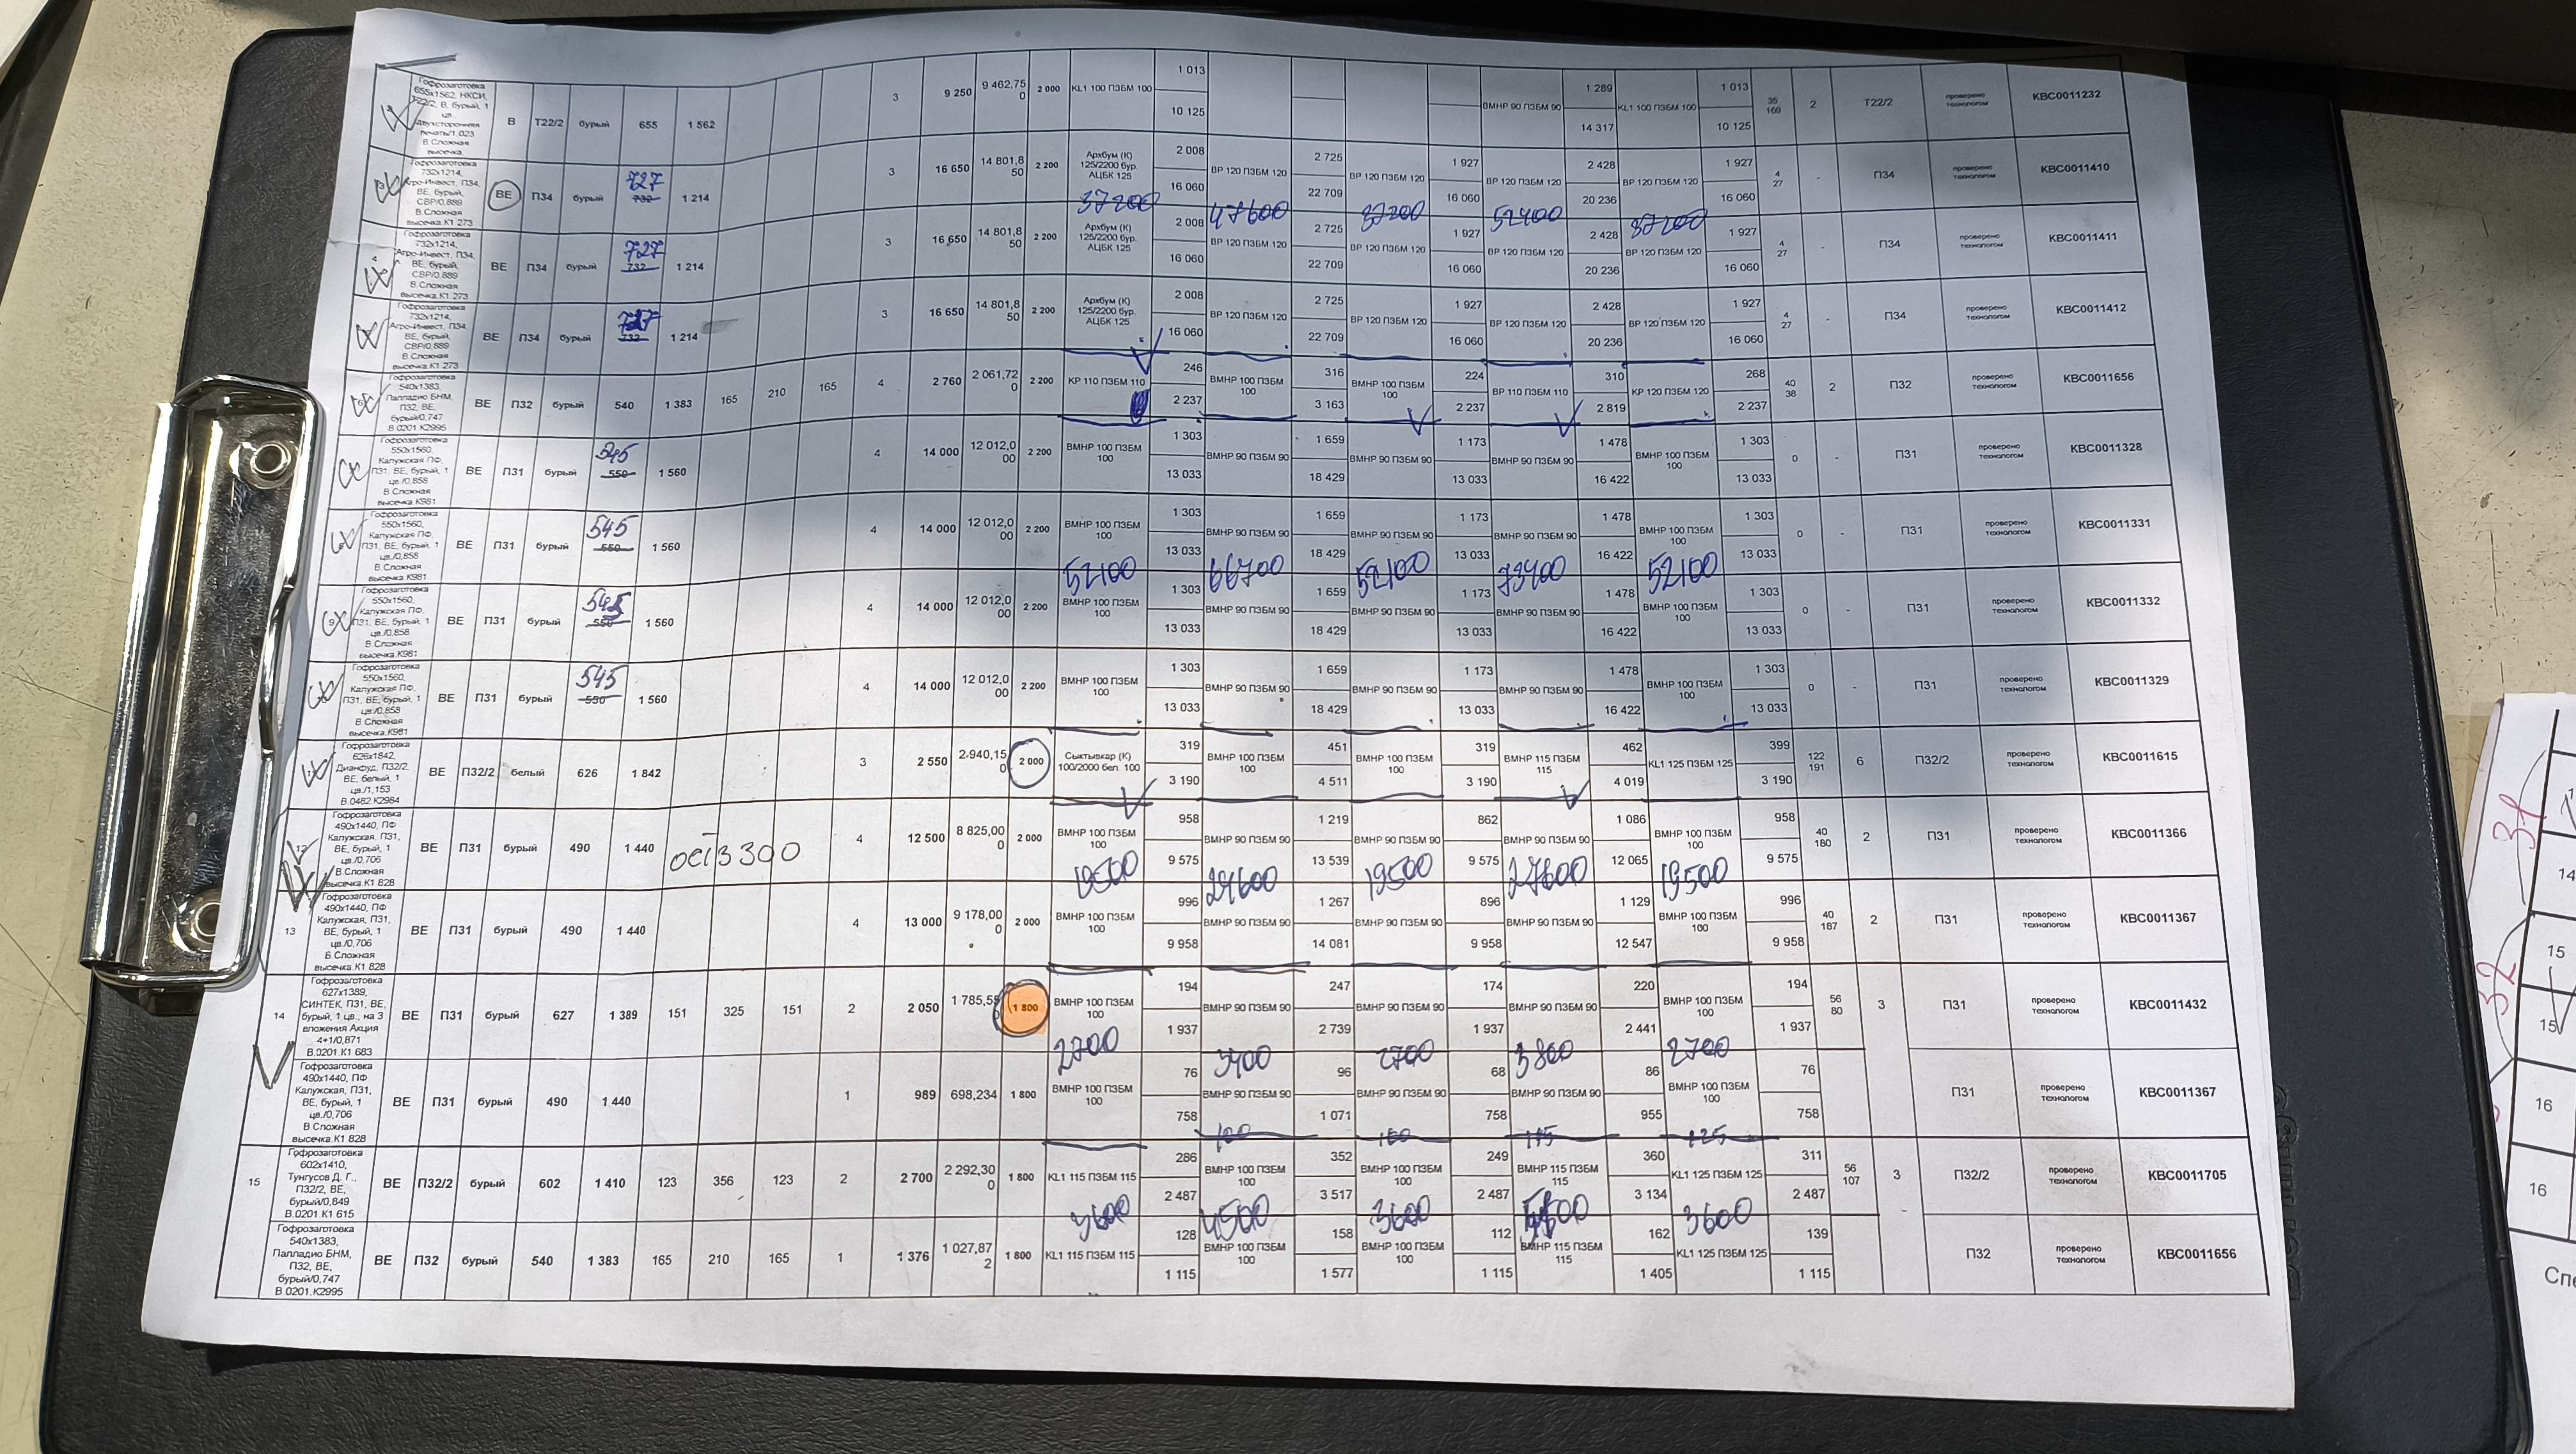
\includegraphics[height=0.38\textheight, keepaspectratio]{Pics/V Задание на ГА.jpg}
\end{center}
 \caption{Задание на ГА}
 \label{pic:Задание на ГА}
\end{figure}

\begin{figure}
\begin{center}
 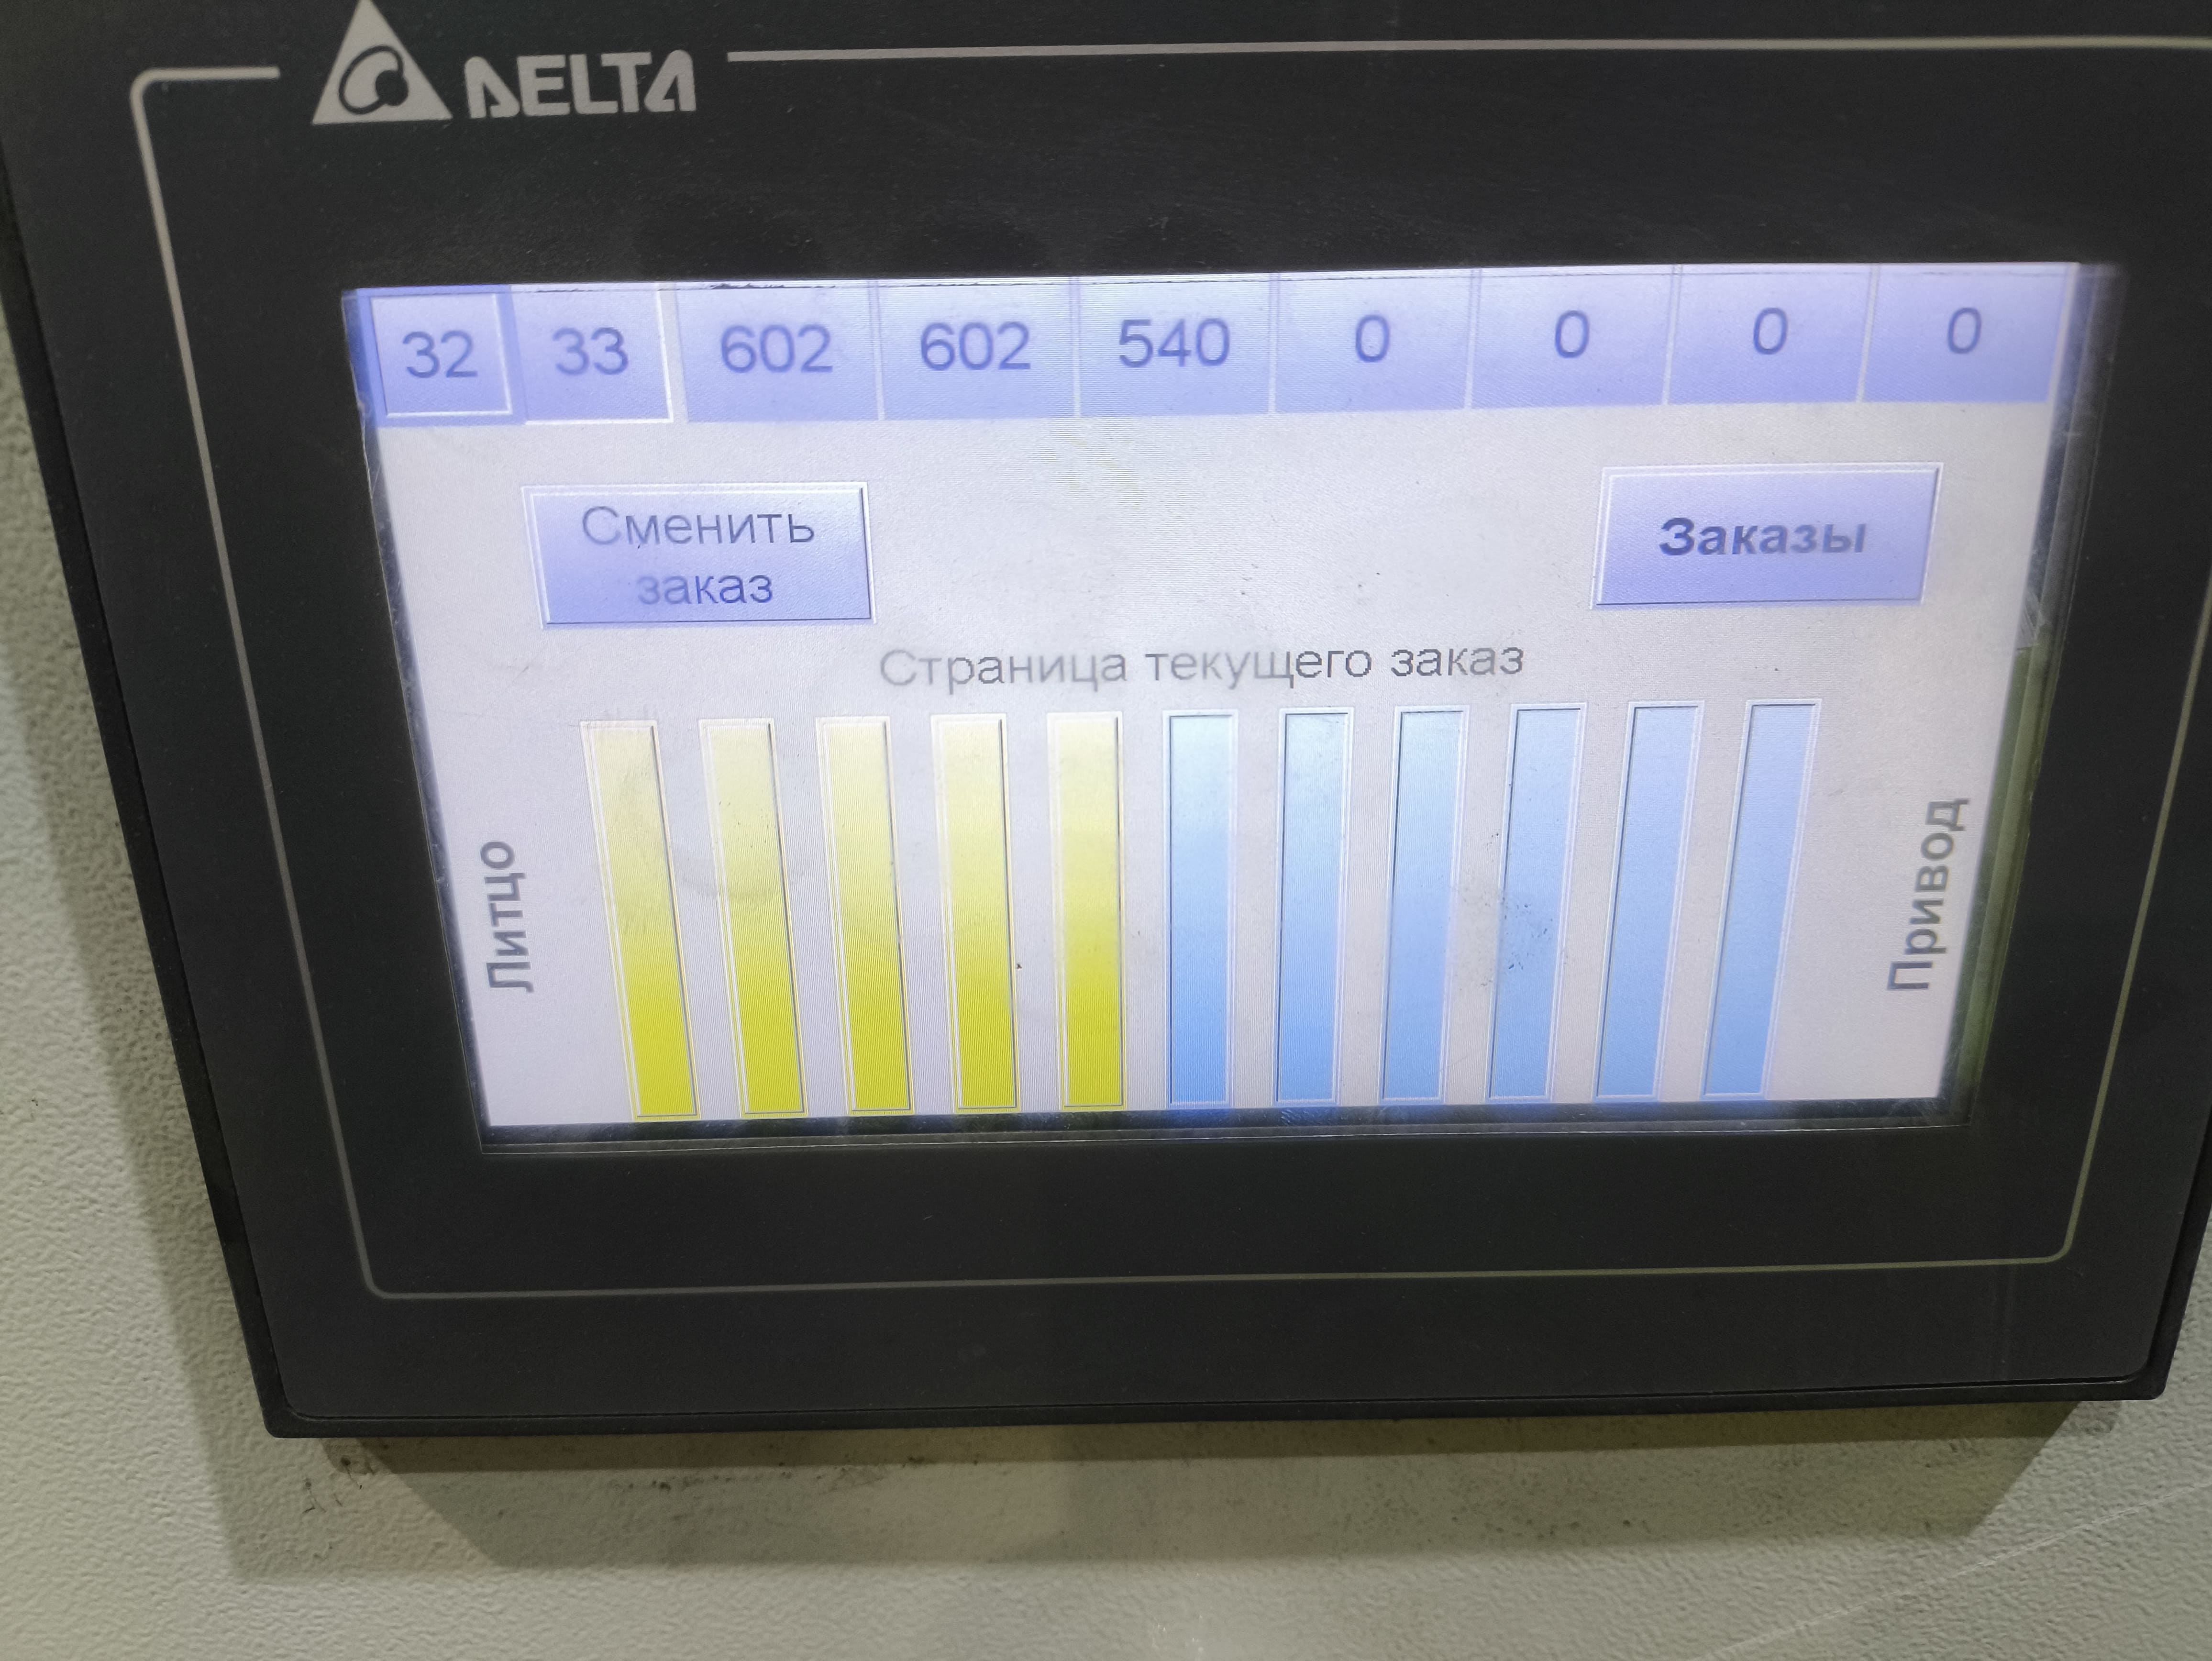
\includegraphics[height=0.38\textheight, keepaspectratio]{Pics/V задание на резке.jpg}
\end{center}
 \caption{Ввод заданий на гофроагрегате}
 \label{pic:V задание на резке}
\end{figure}

\begin{figure}
\begin{center}
 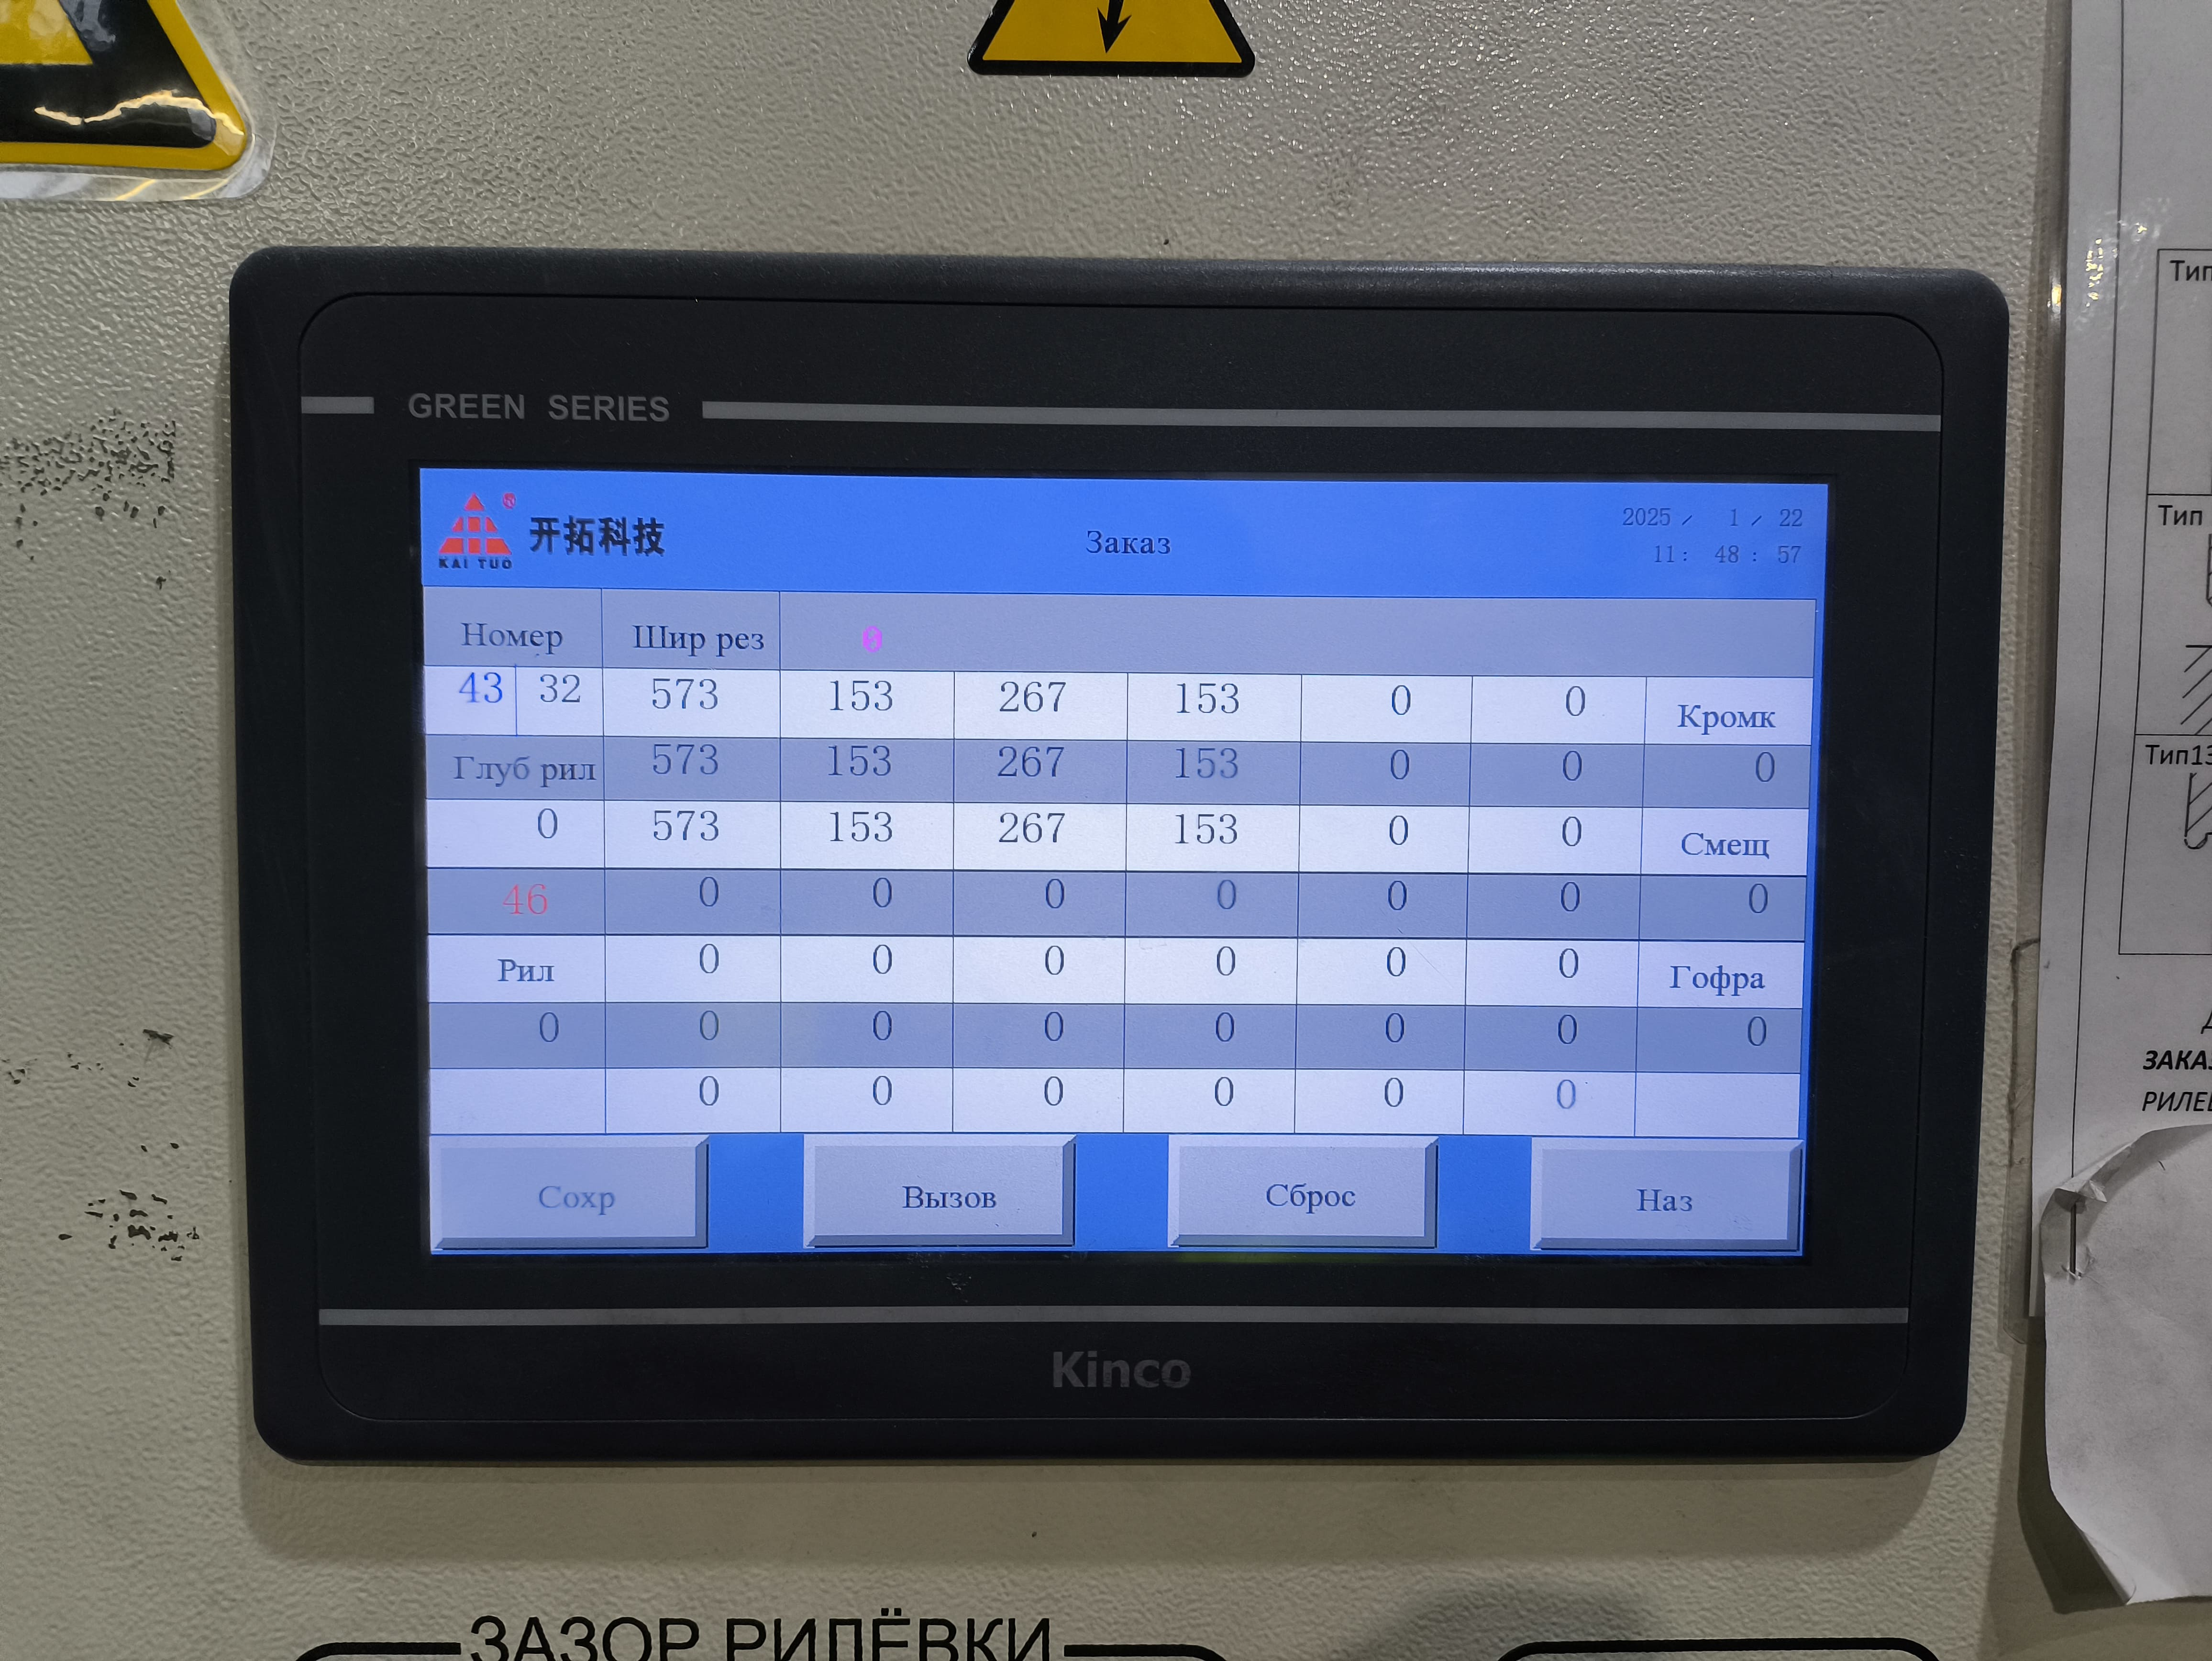
\includegraphics[height=0.38\textheight, keepaspectratio]{Pics/V задание рилевки.jpg}
\end{center}
 \caption{Ввод заданий на гофроагрегате}
 \label{pic:V задание рилевки}
\end{figure}

\begin{figure}
\begin{center}
 \includegraphics[height=0.4
 \textheight, keepaspectratio]{Pics/Vвнесениевыработки.jpg}
\end{center}
 \caption{Внесение факта выработки}
 \label{pic:Vвнесениевыработки}
\end{figure}

\begin{figure}
\begin{center}
 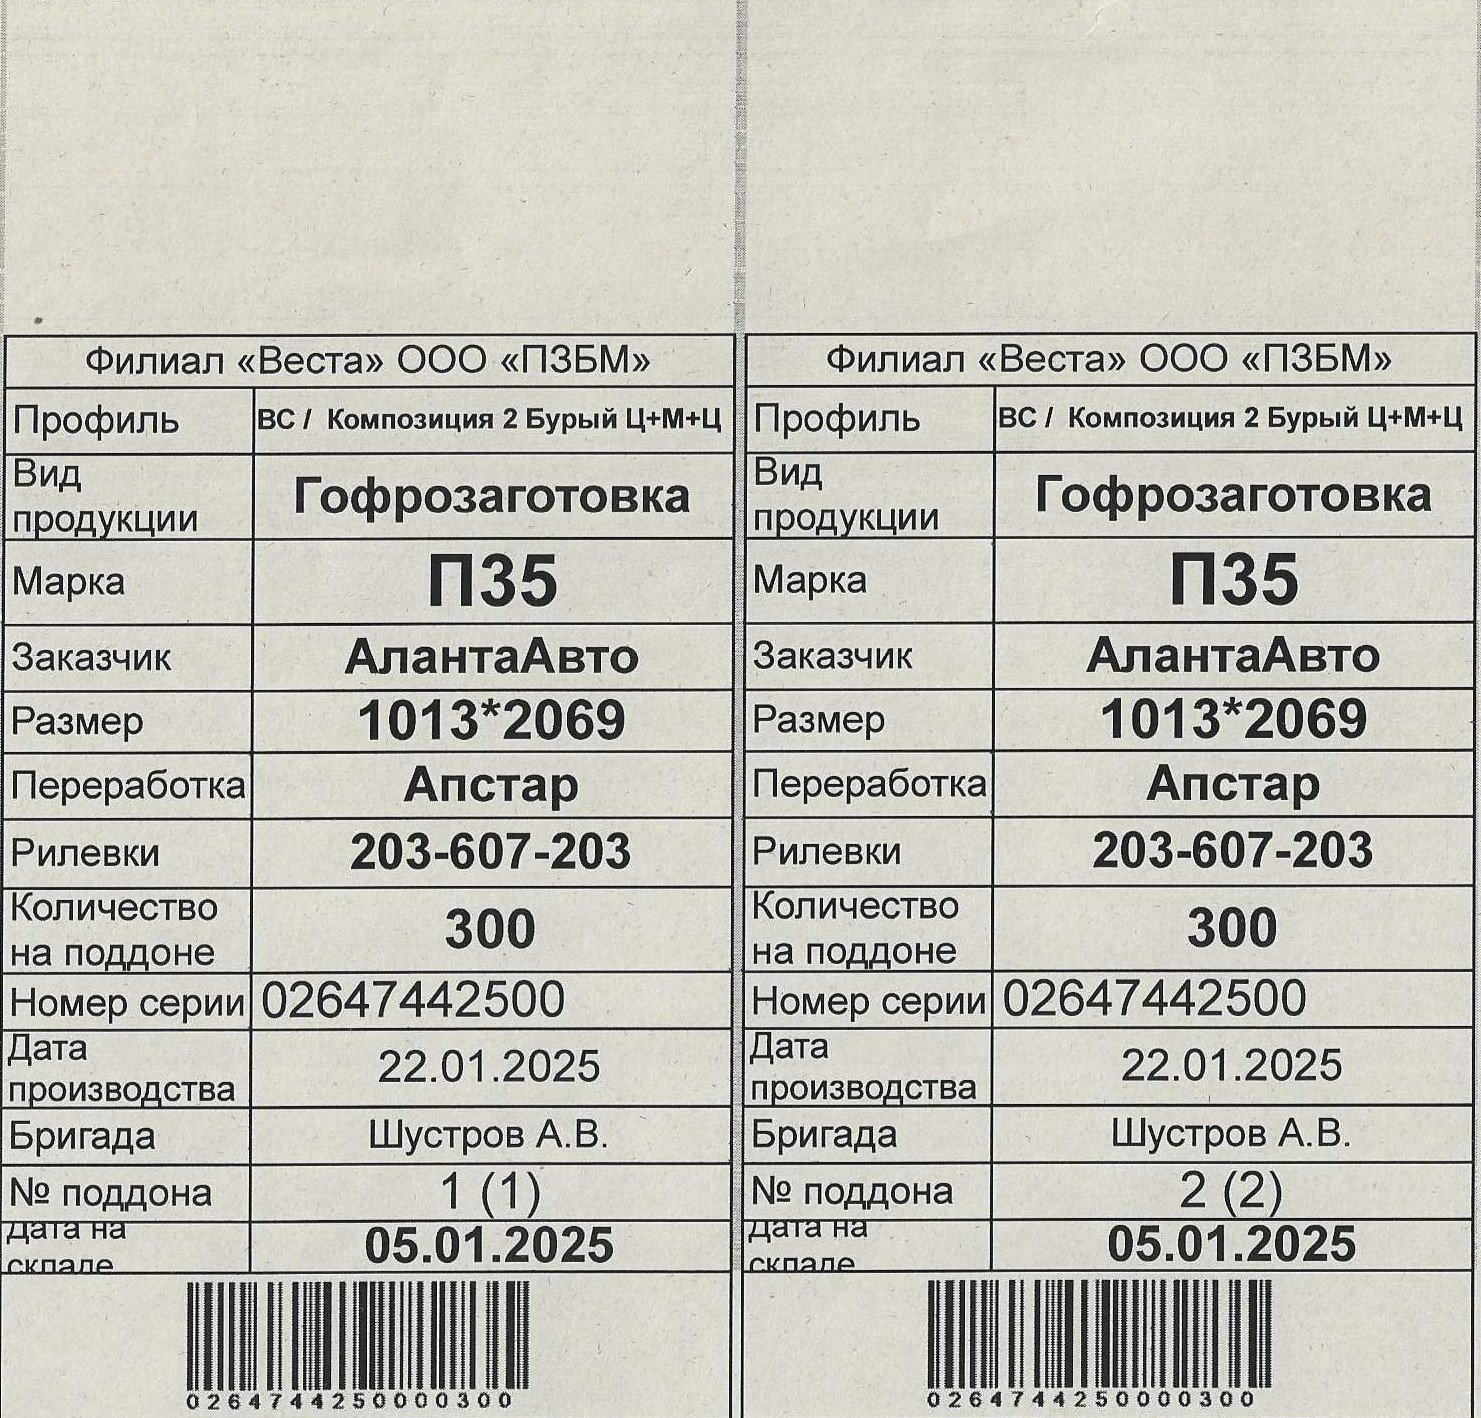
\includegraphics[height=0.6\textheight, keepaspectratio]{Pics/V.10.jpg}
\end{center}
 \caption{Бирки на полуфабрикаты}
 \label{pic:V.10}
\end{figure}

\begin{figure}
\begin{center}
 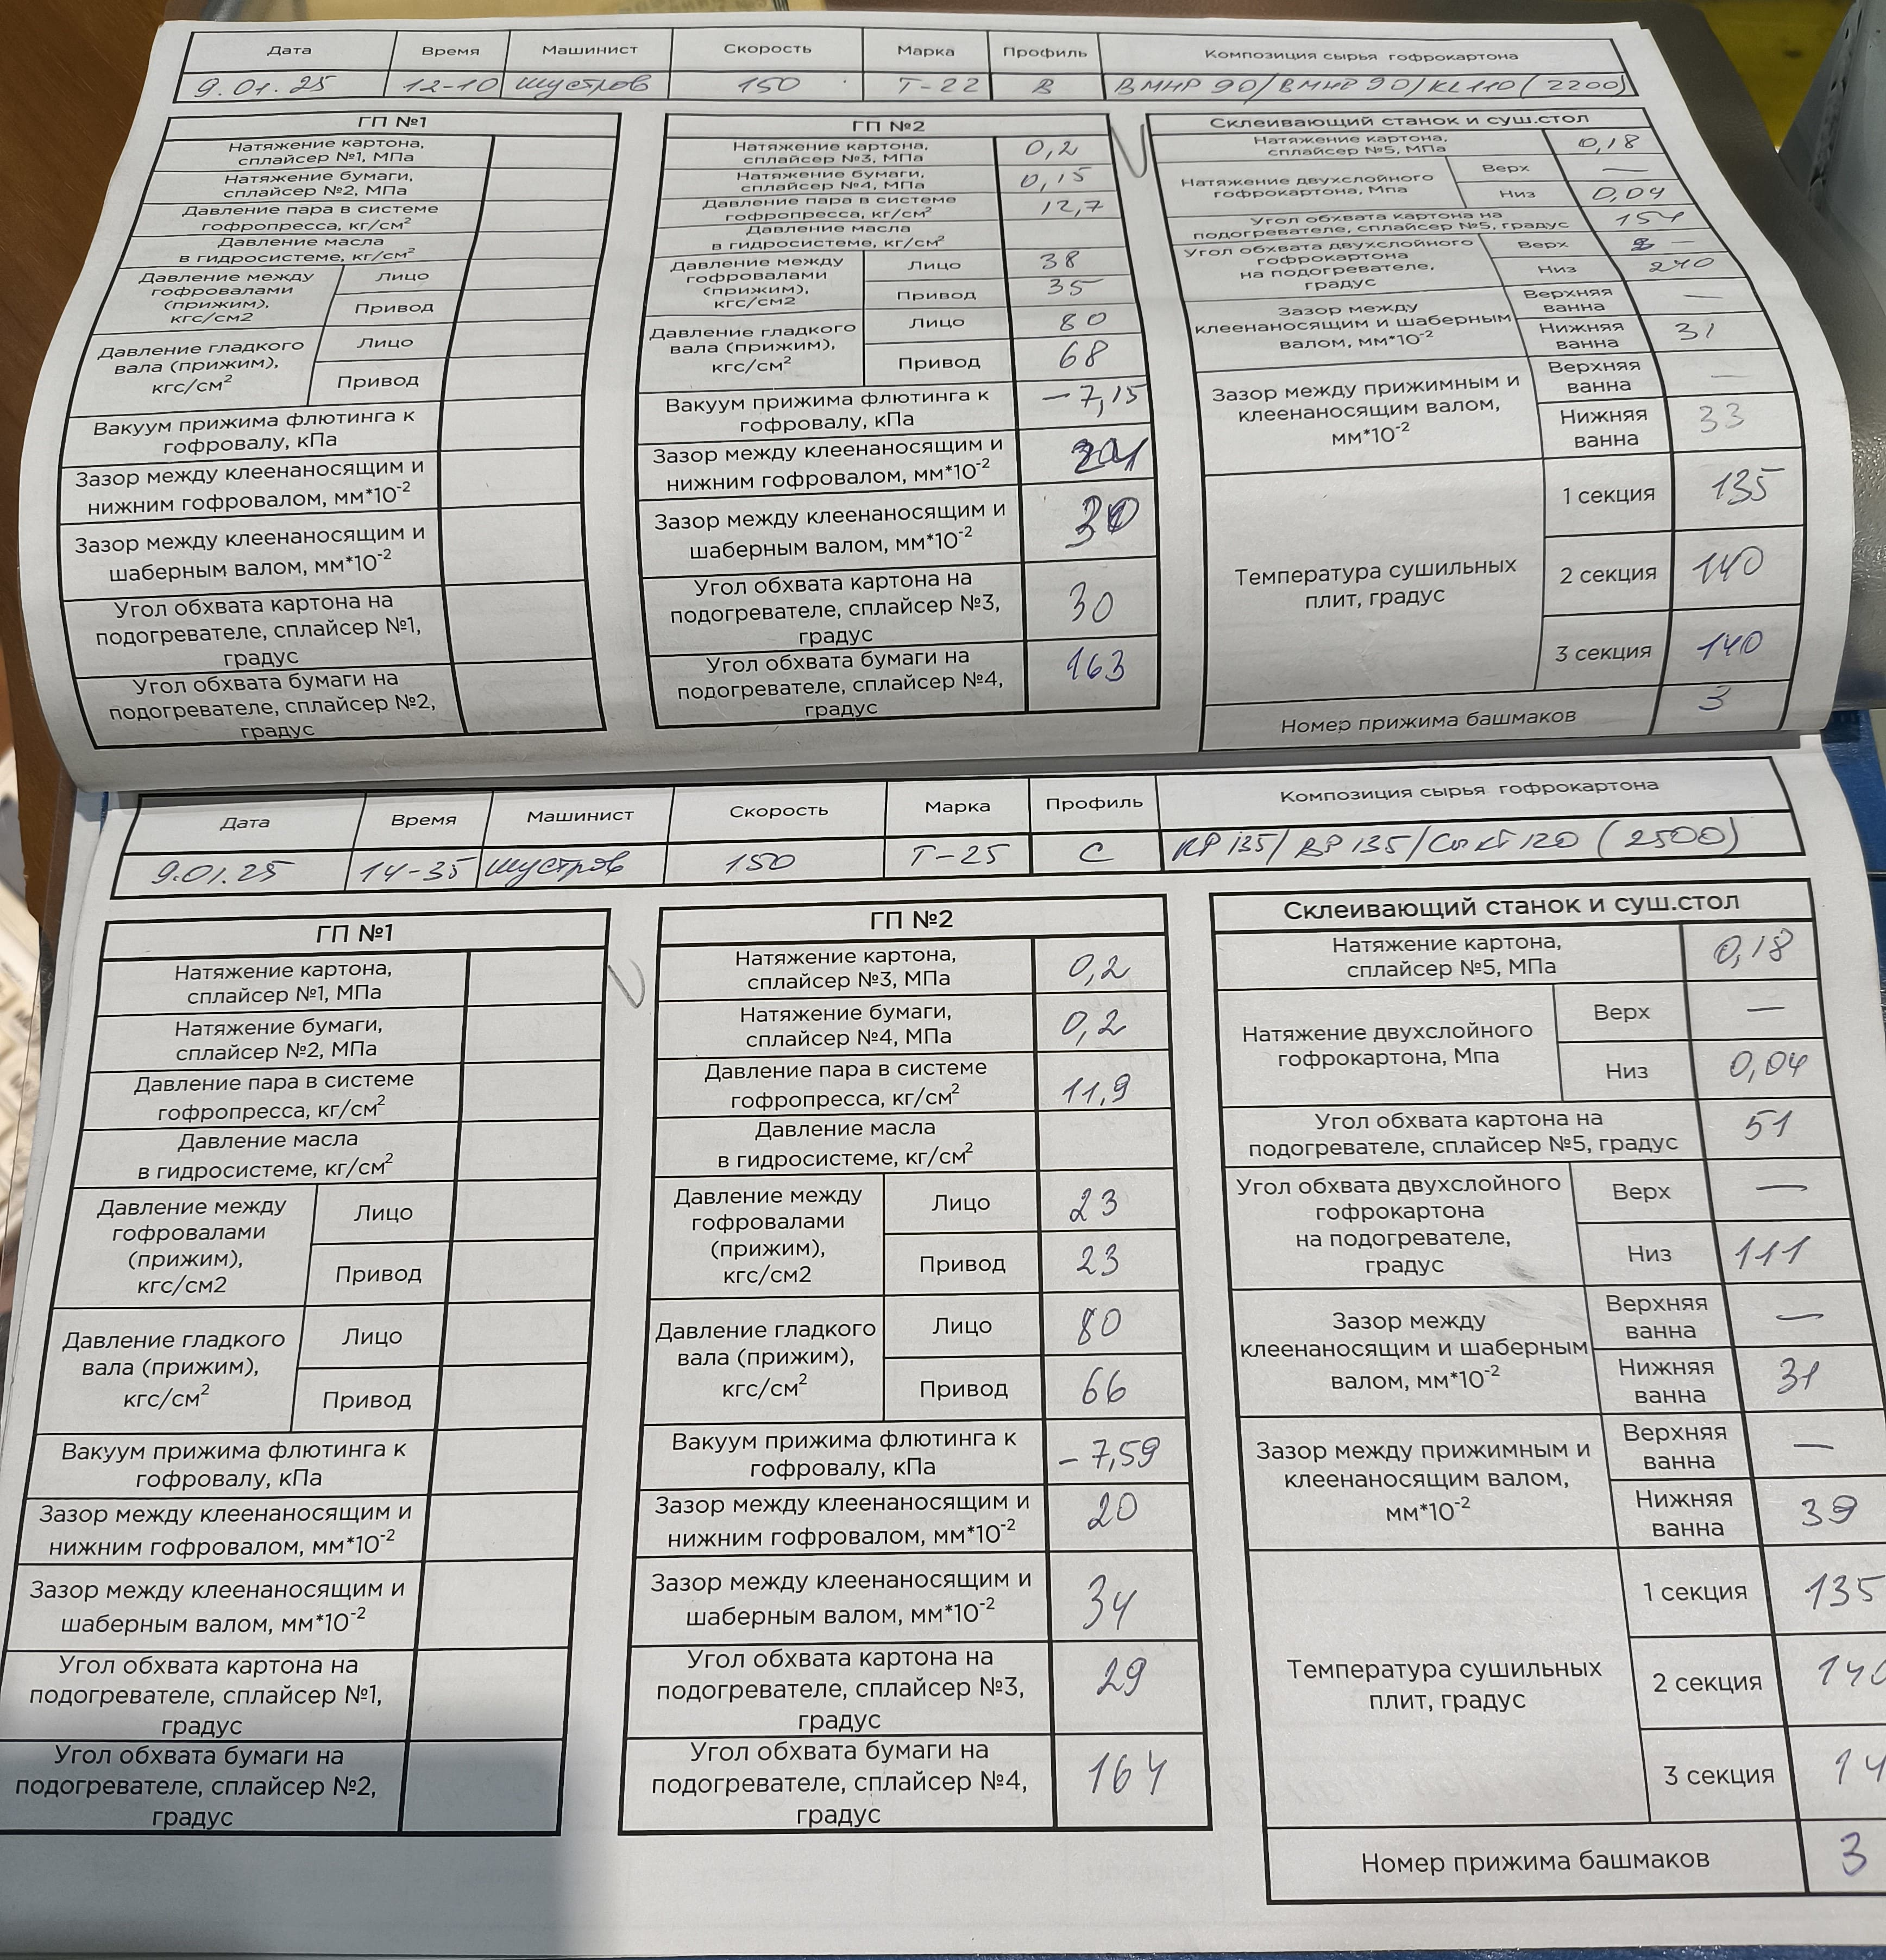
\includegraphics[height=0.7\textheight, keepaspectratio]{Pics/V журнал техн параметров.jpg}
\end{center}
 \caption{Журнал технологических параметров}
 \label{pic:V журнал техн параметров}
\end{figure}

\begin{figure}
\begin{center}
 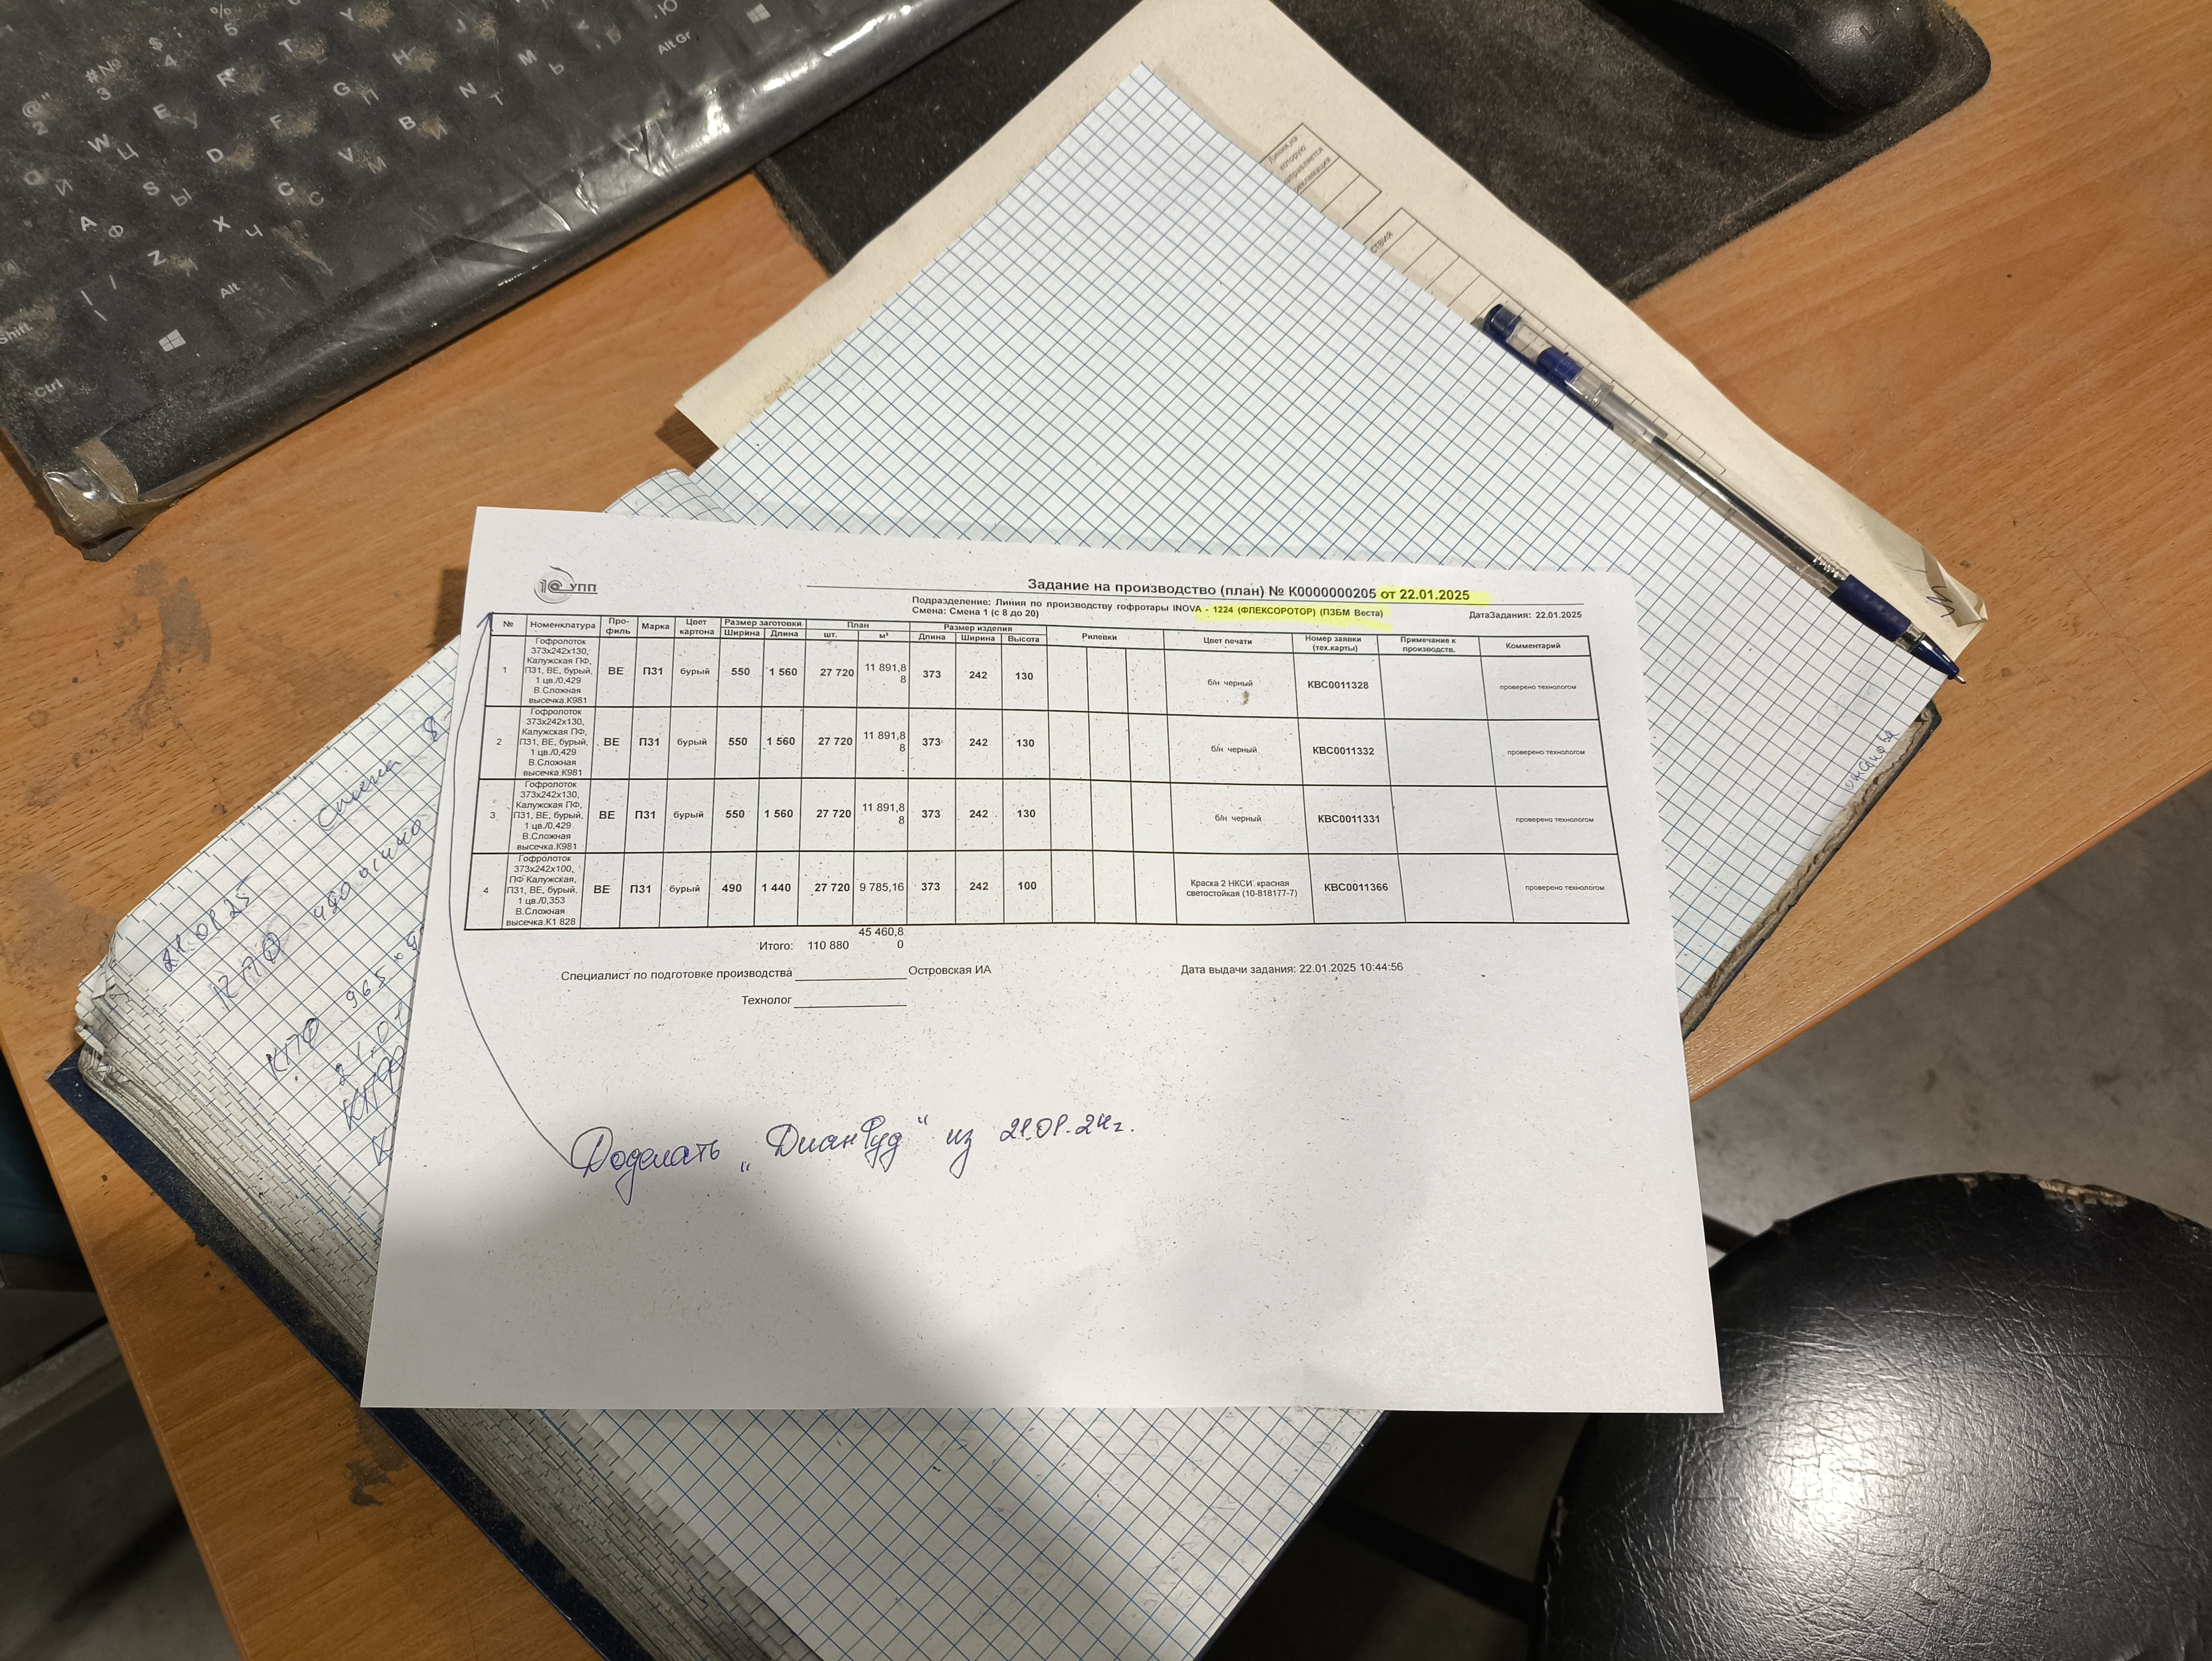
\includegraphics[height=0.5\textheight, keepaspectratio]{Pics/VI задание для переработки.jpg}
\end{center}
 \caption{Задание на линию переработки}
 \label{pic:VI задание для переработки}
\end{figure}

\begin{figure}
\begin{center}
 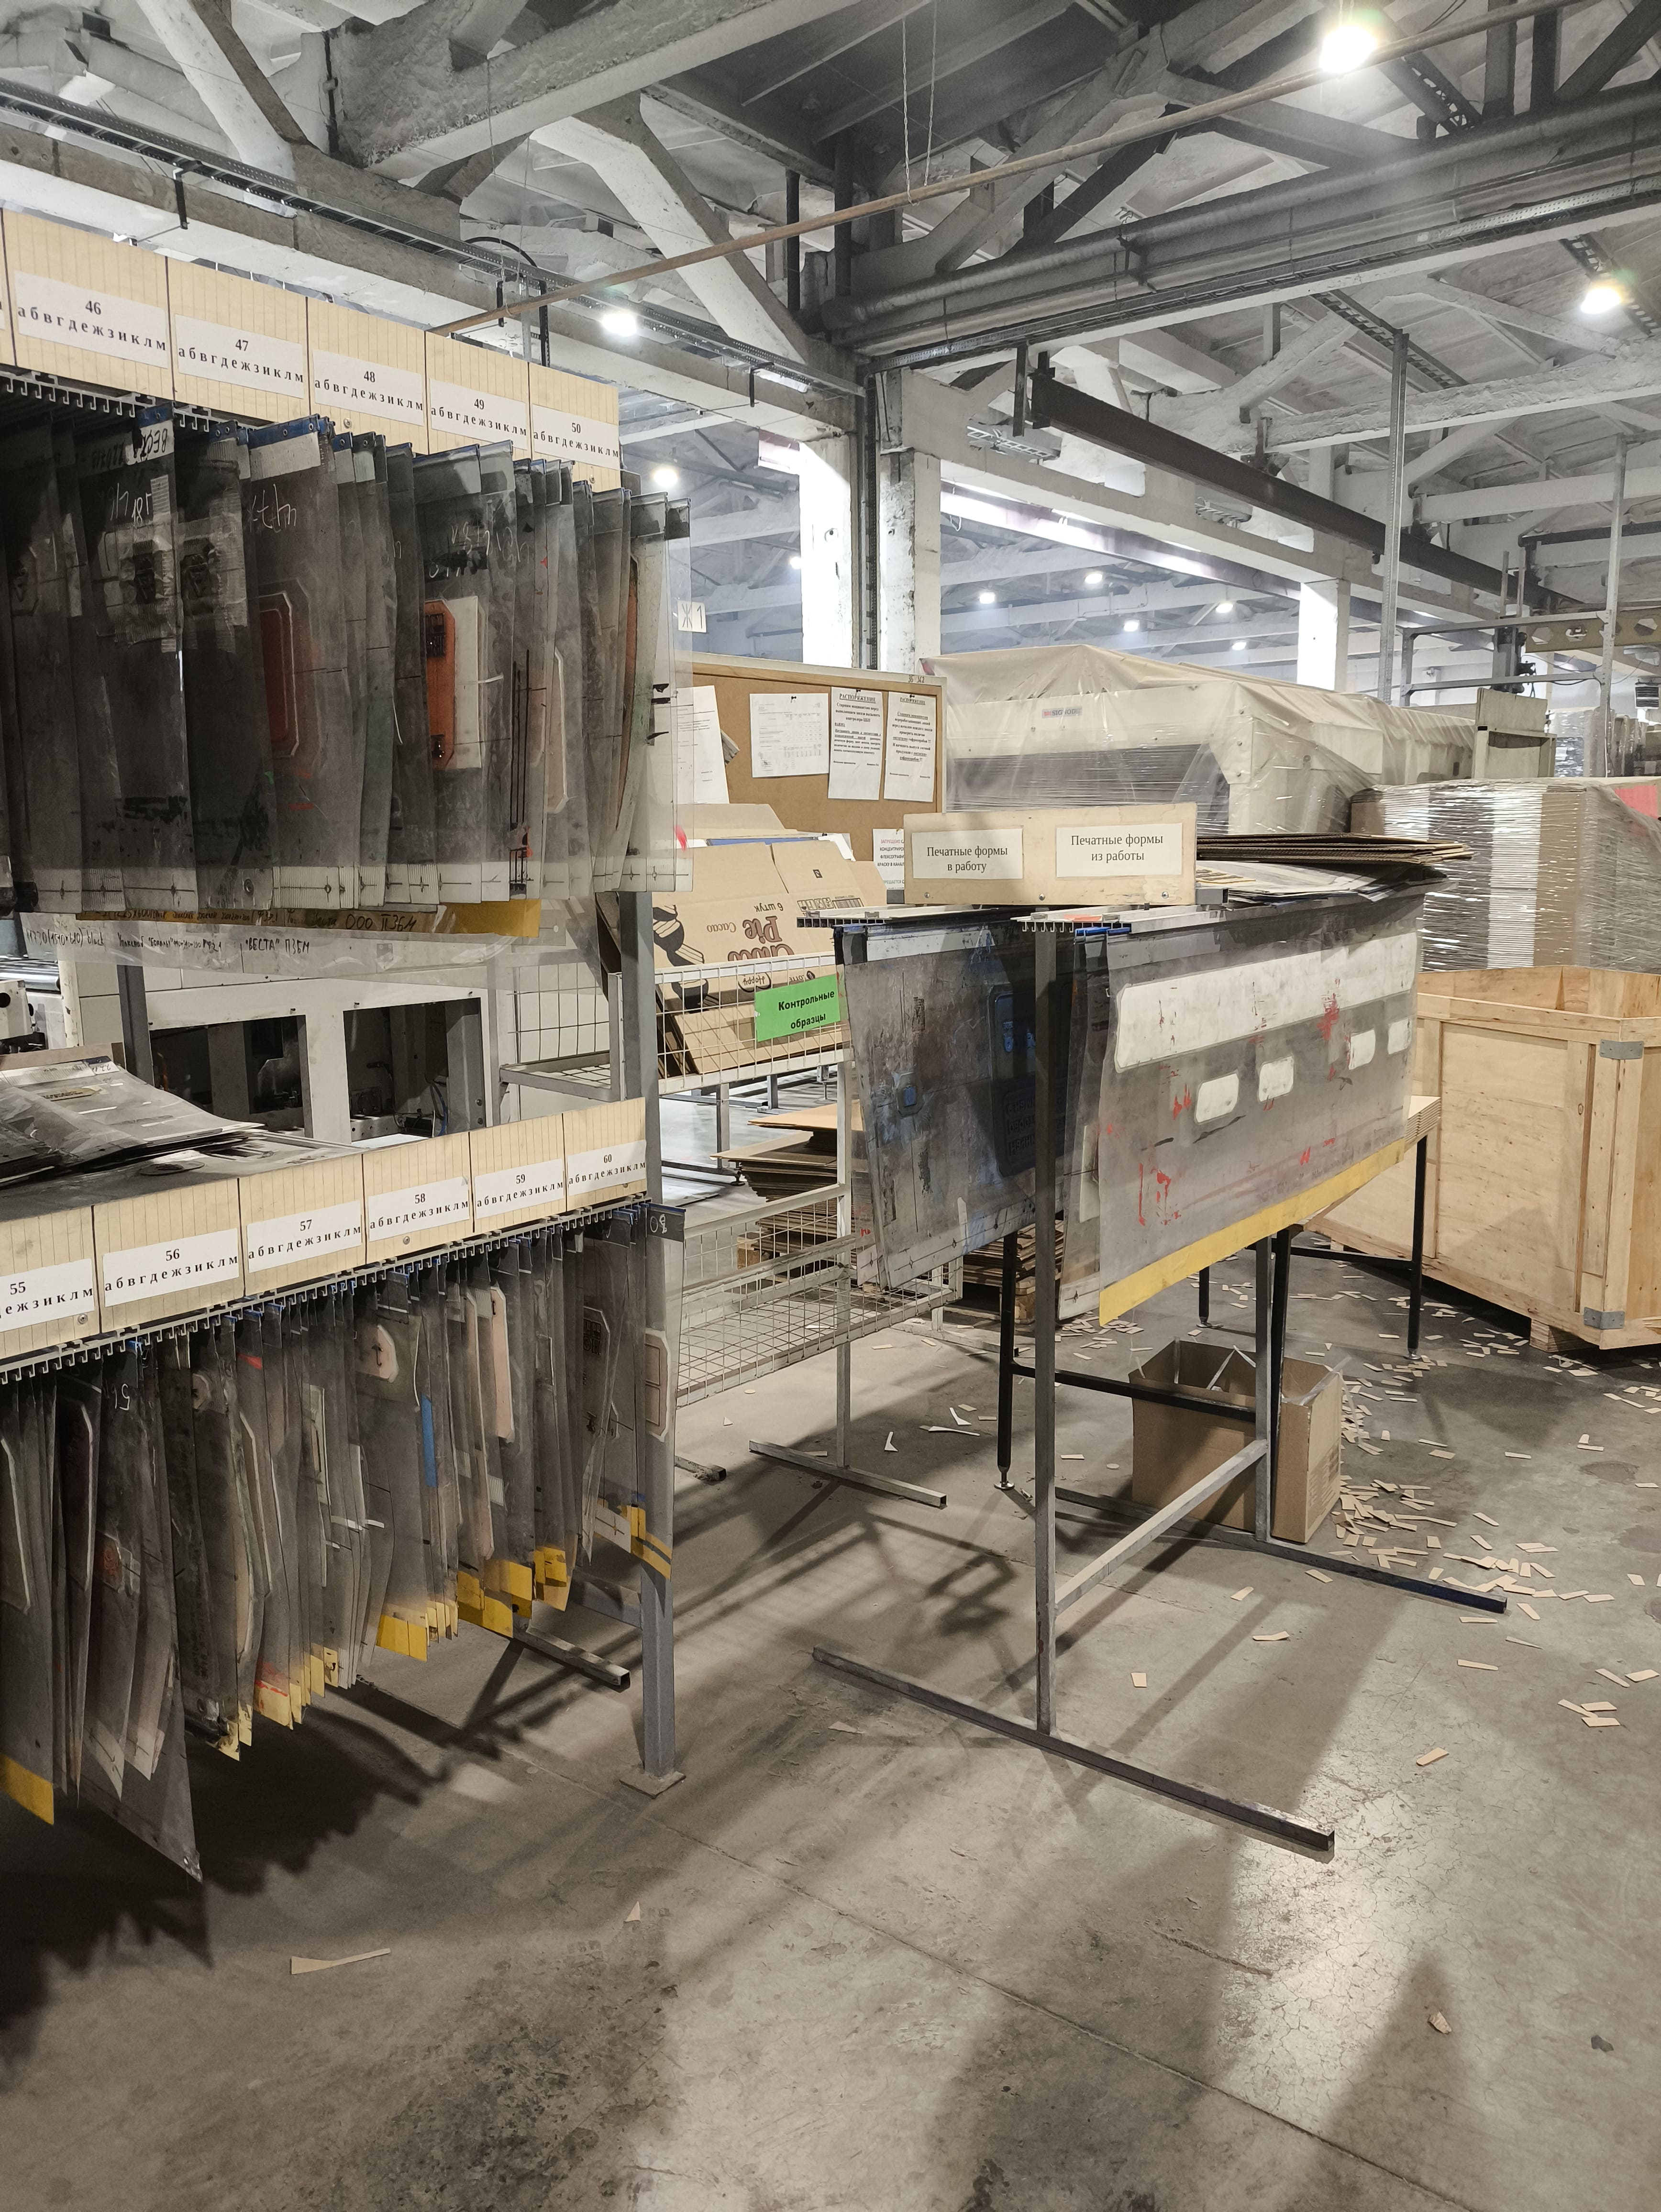
\includegraphics[height=0.8\textheight, keepaspectratio]{Pics/II хранение фпф.jpg}
\end{center}
 \caption{Оснастка у линий переработки}
 \label{pic:II хранение фпф}
\end{figure}

\begin{figure}
\begin{center}
 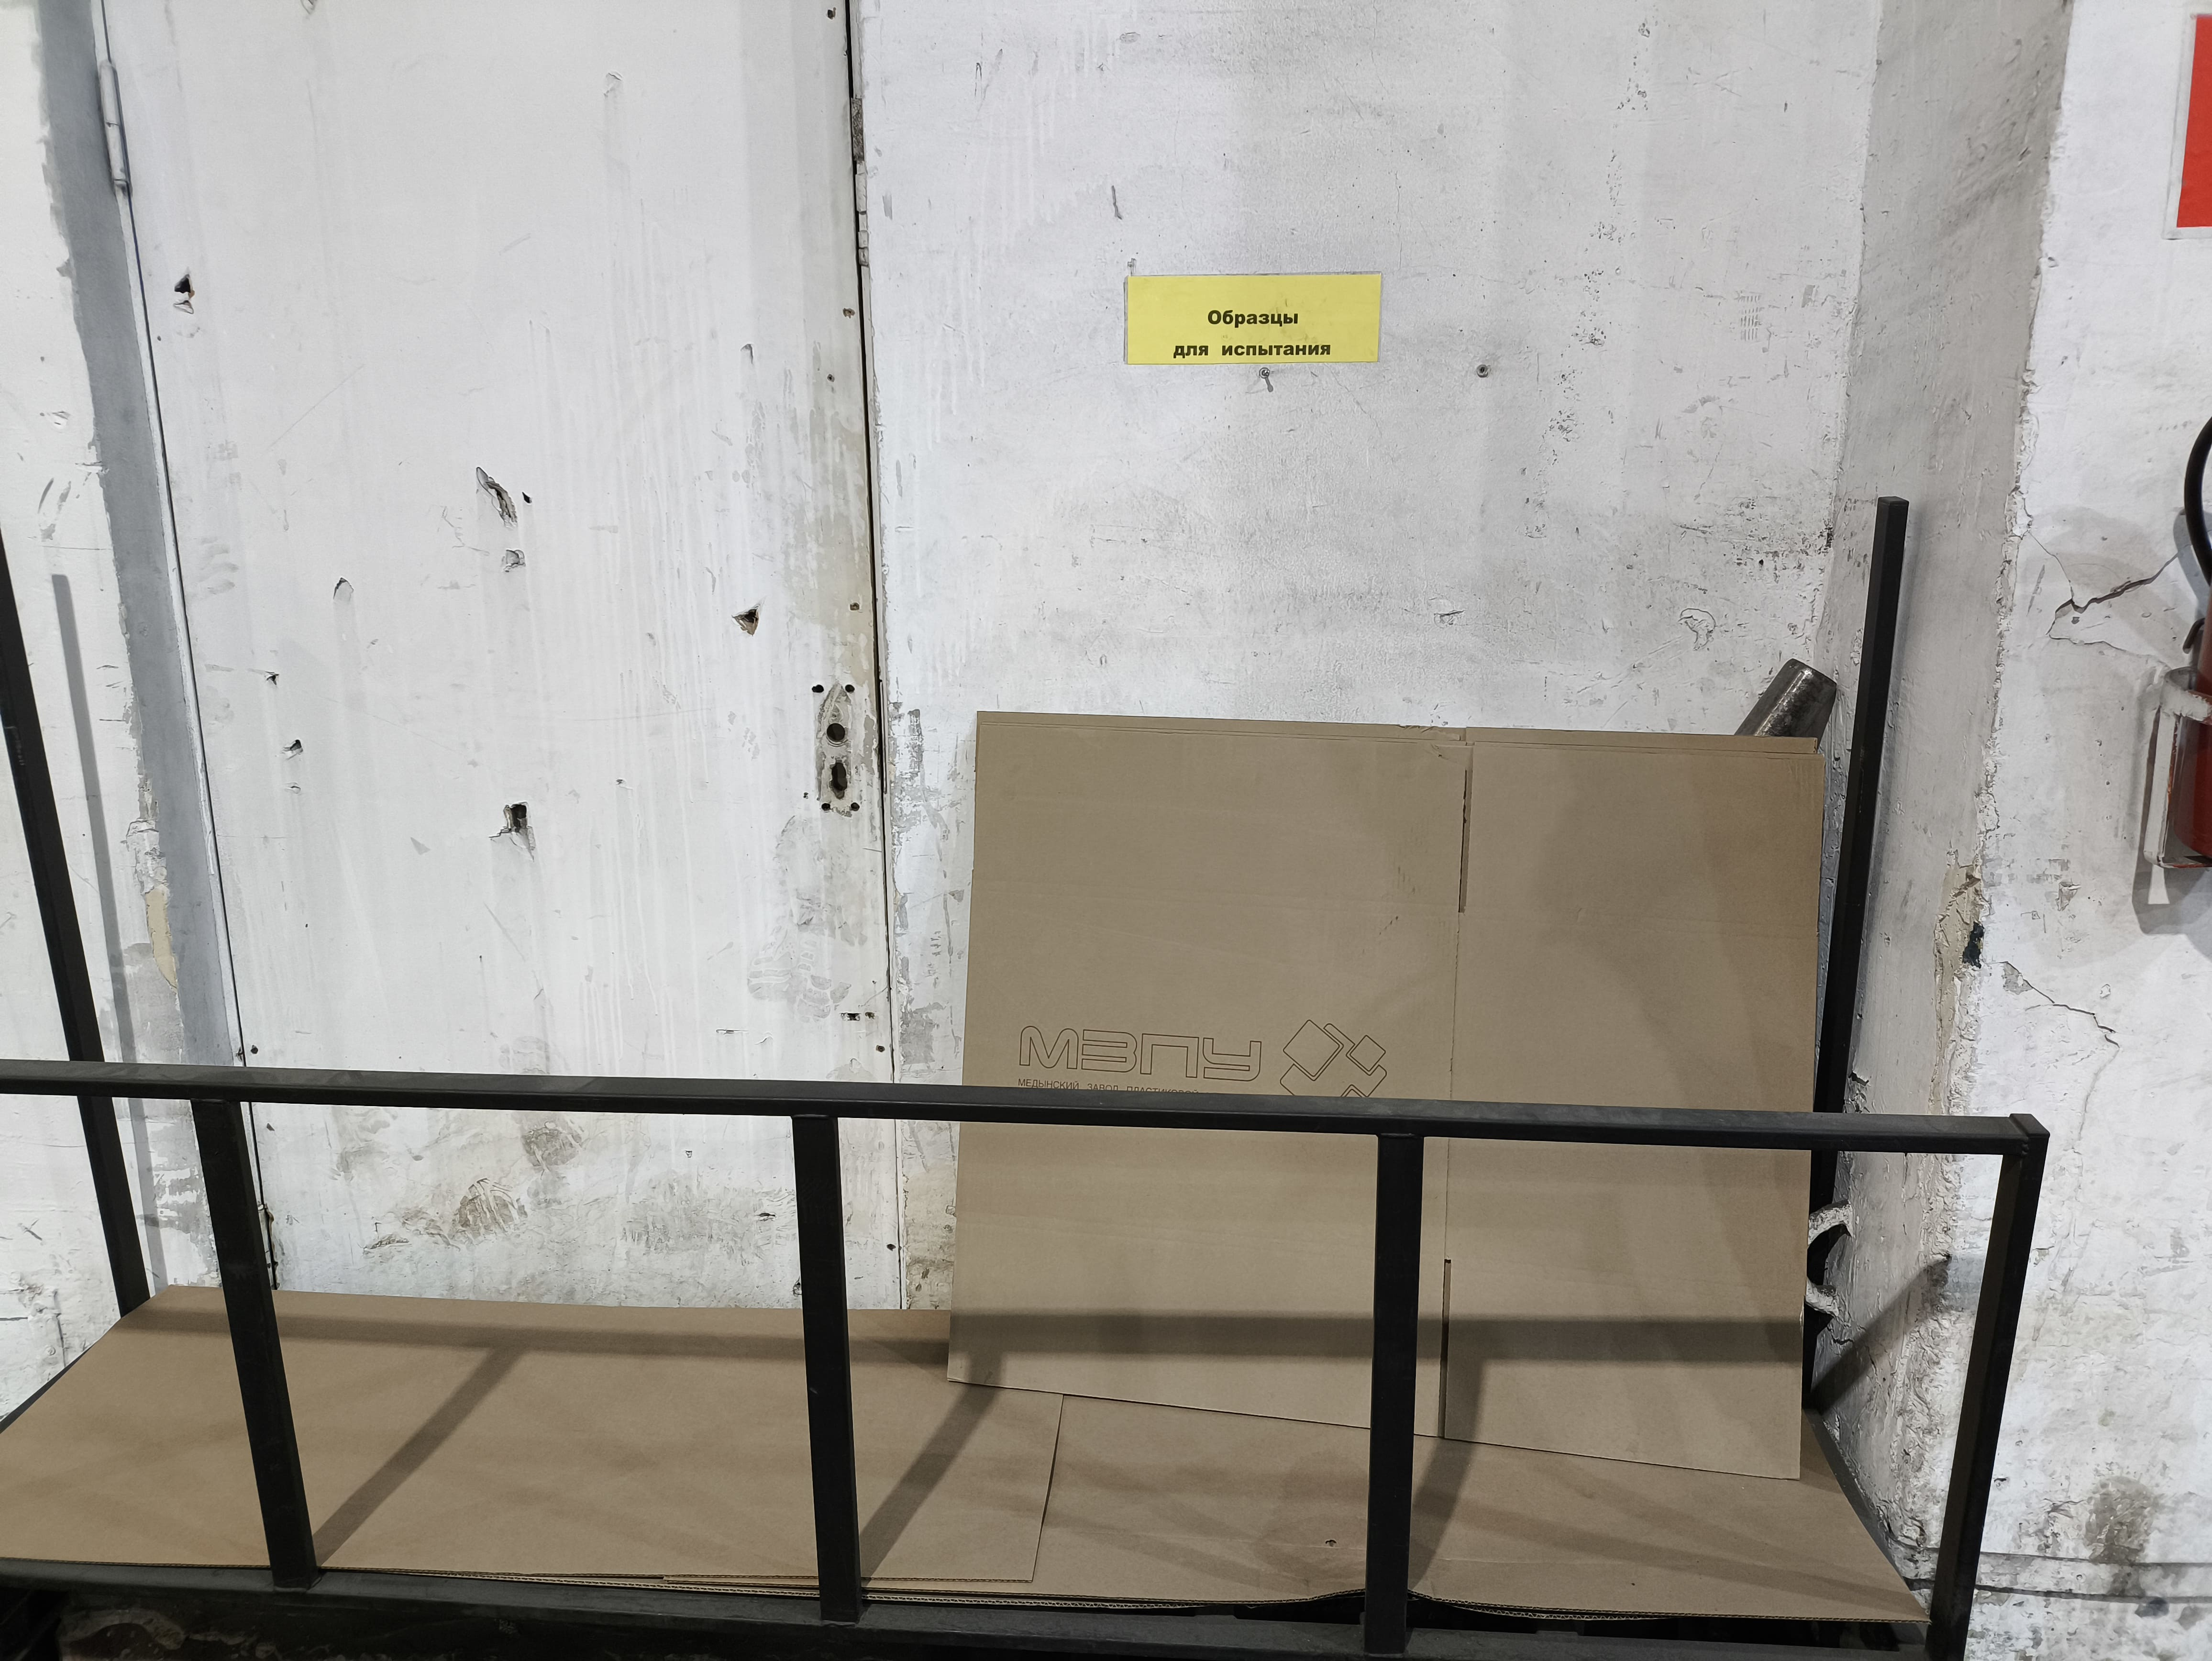
\includegraphics[height=0.5\textheight, keepaspectratio]{Pics/V образцы для ОТК.jpg}
\end{center}
 \caption{Образцы для ОУК}
 \label{pic:V образцы для ОТК}
\end{figure}

\begin{figure}
\begin{center}
 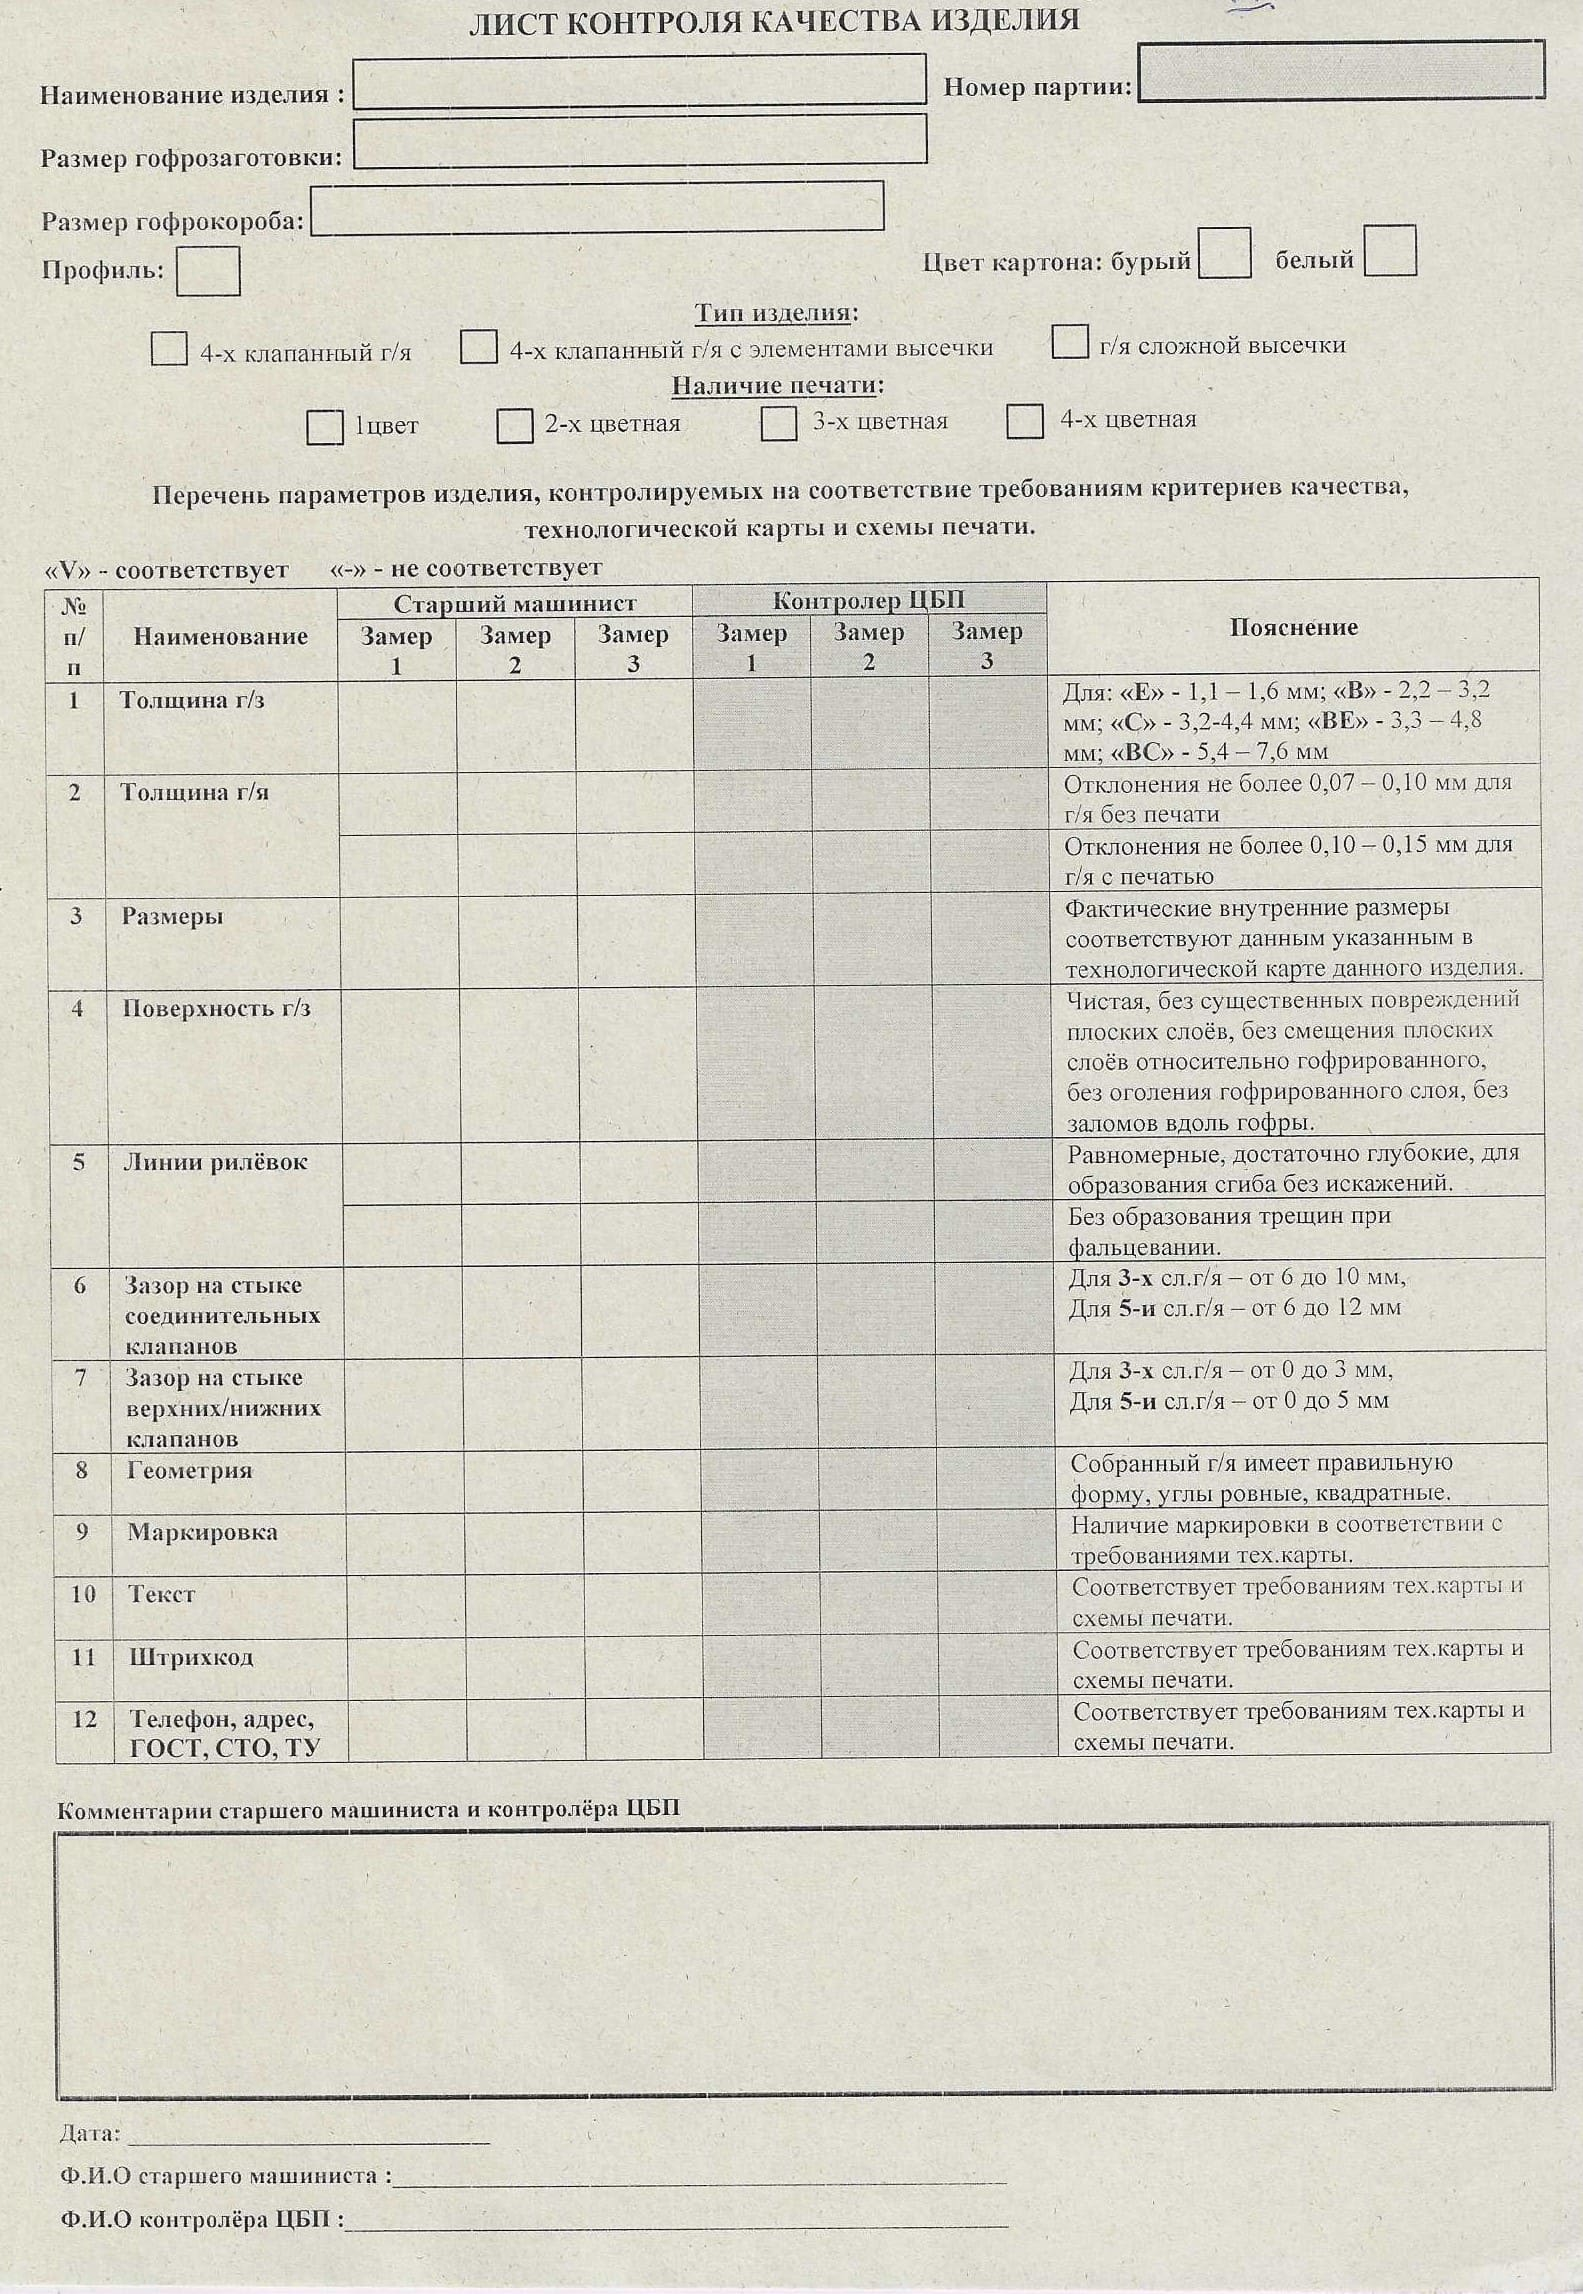
\includegraphics[height=0.9\textheight, keepaspectratio]{Pics/VI.jpg}
\end{center}
 \caption{Лист контроля качества}
 \label{pic:VI}
\end{figure}

\begin{figure}
\begin{center}
 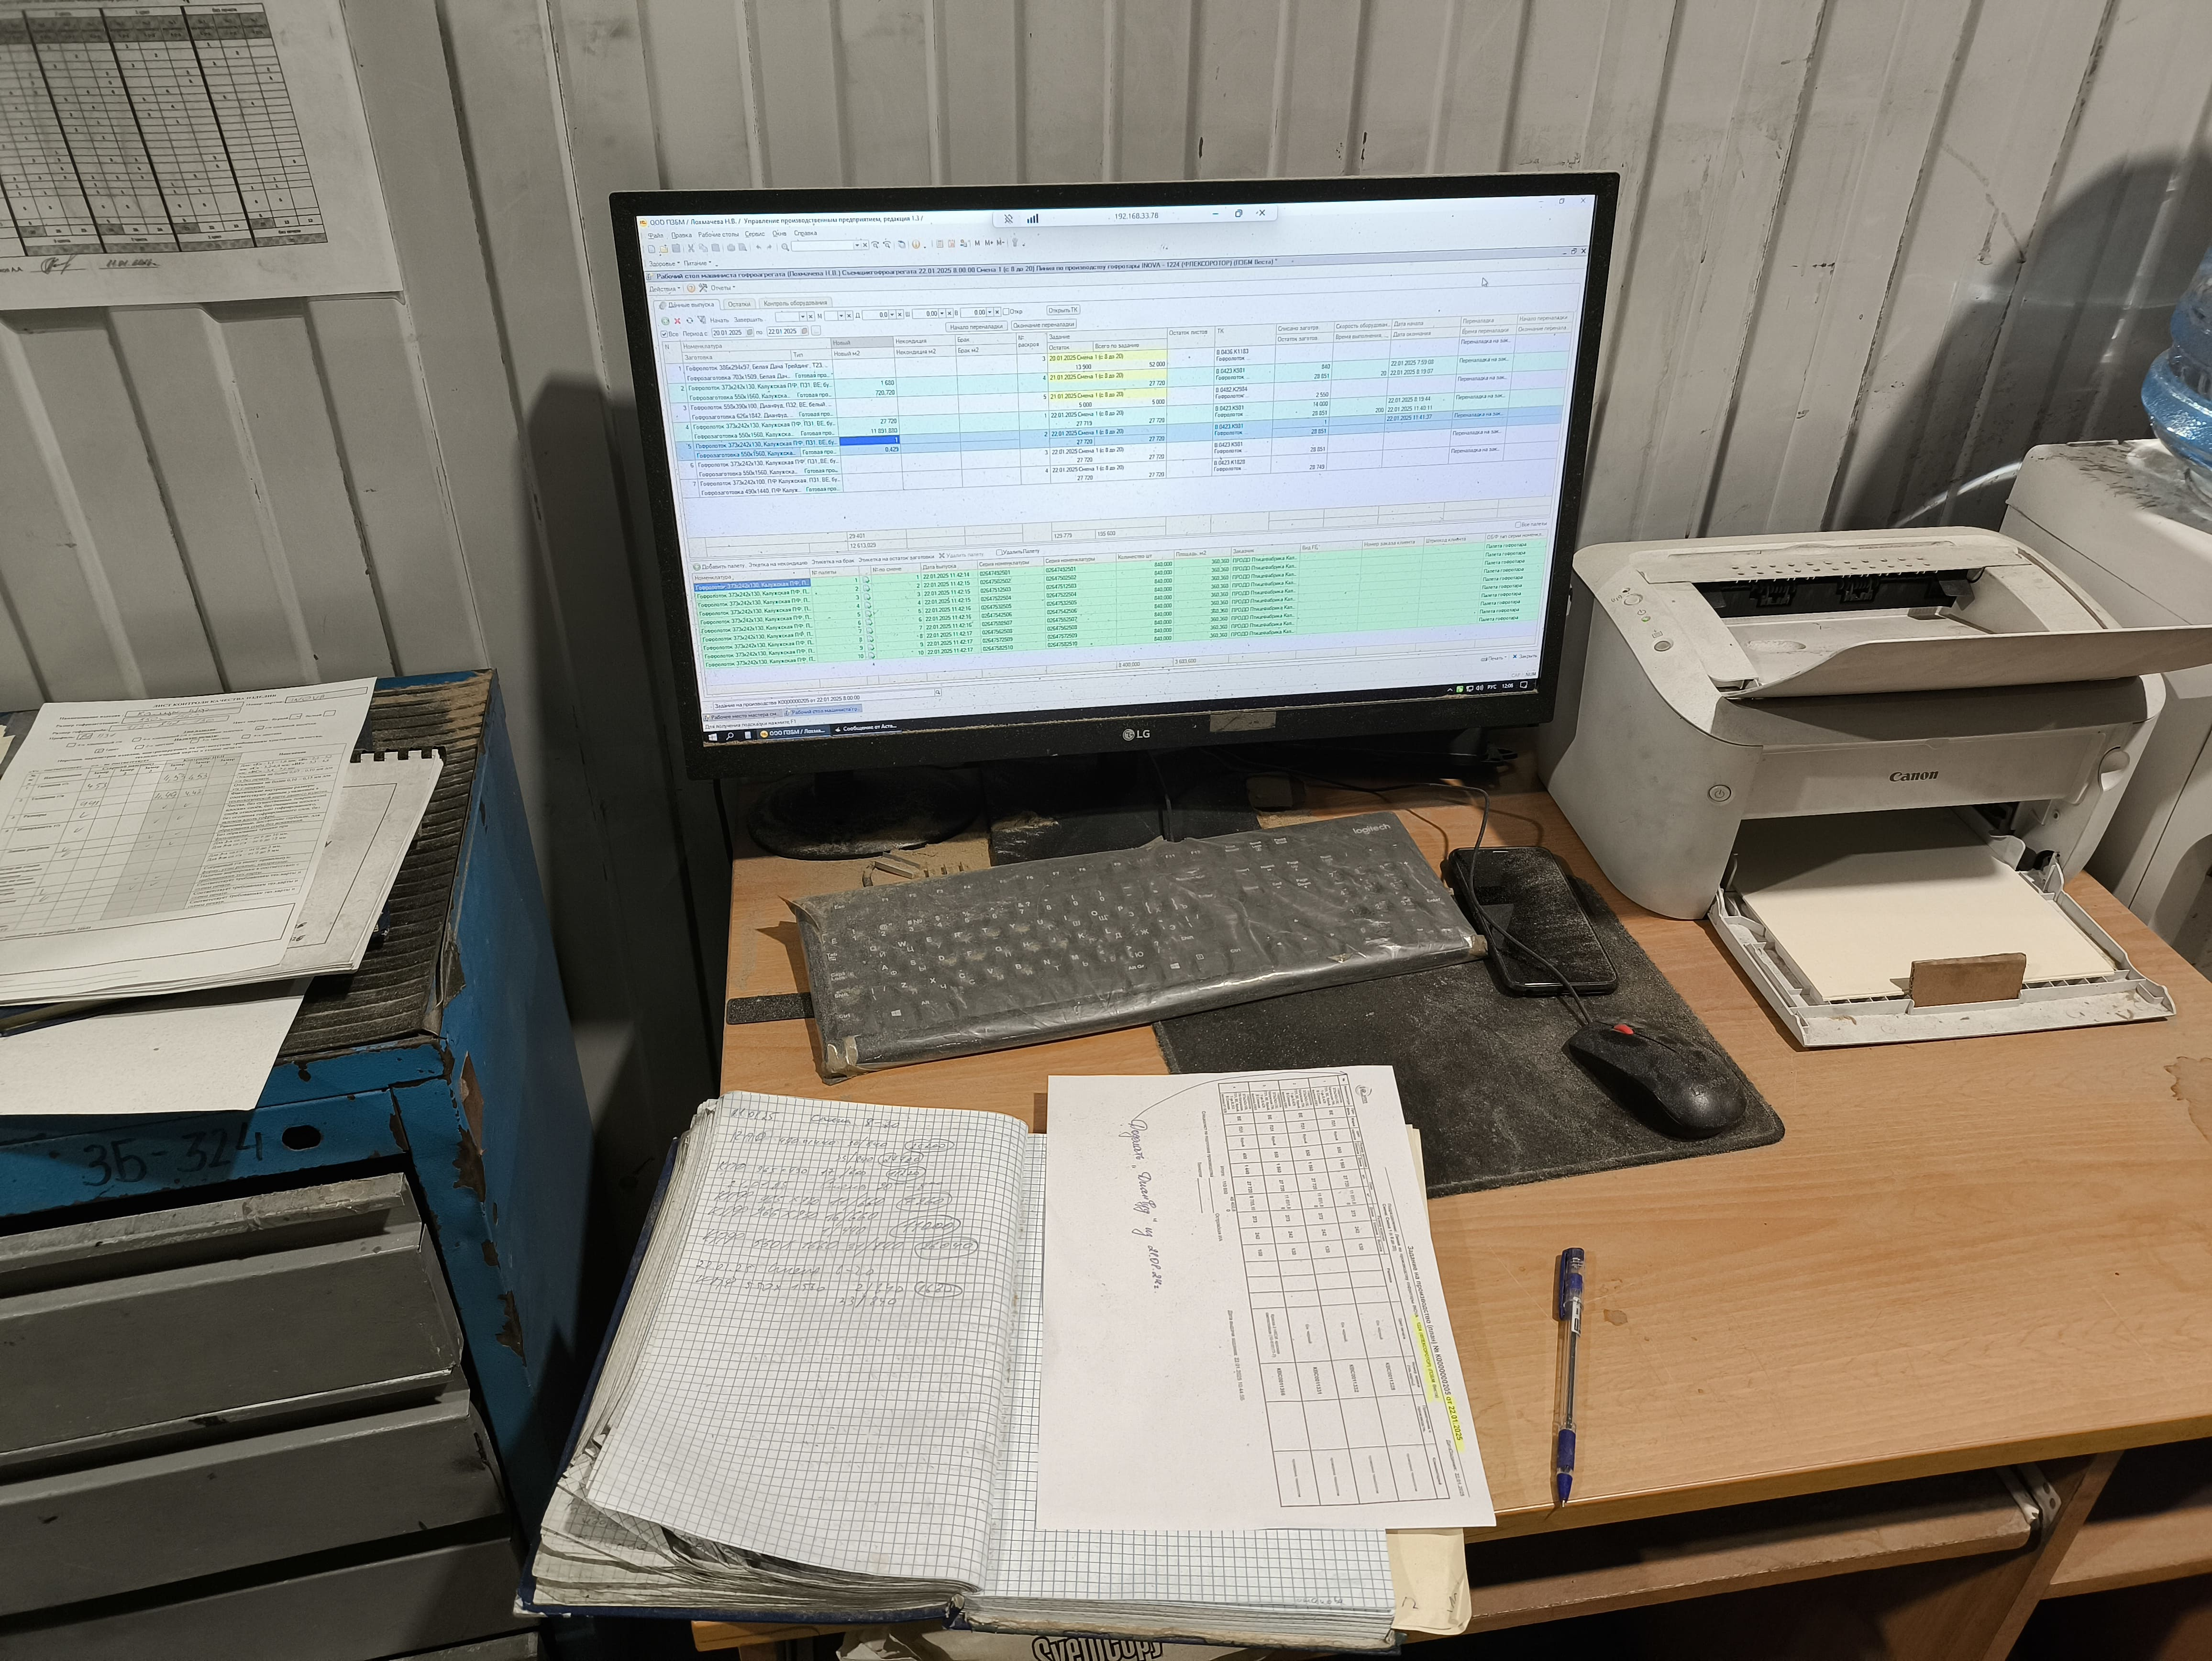
\includegraphics[height=0.5\textheight, keepaspectratio]{Pics/VI рабочее место машиниста.jpg}
\end{center}
 \caption{Внесение факта выработки}
 \label{pic:VI рабочее место машиниста}
\end{figure}

\begin{figure}
\begin{center}
 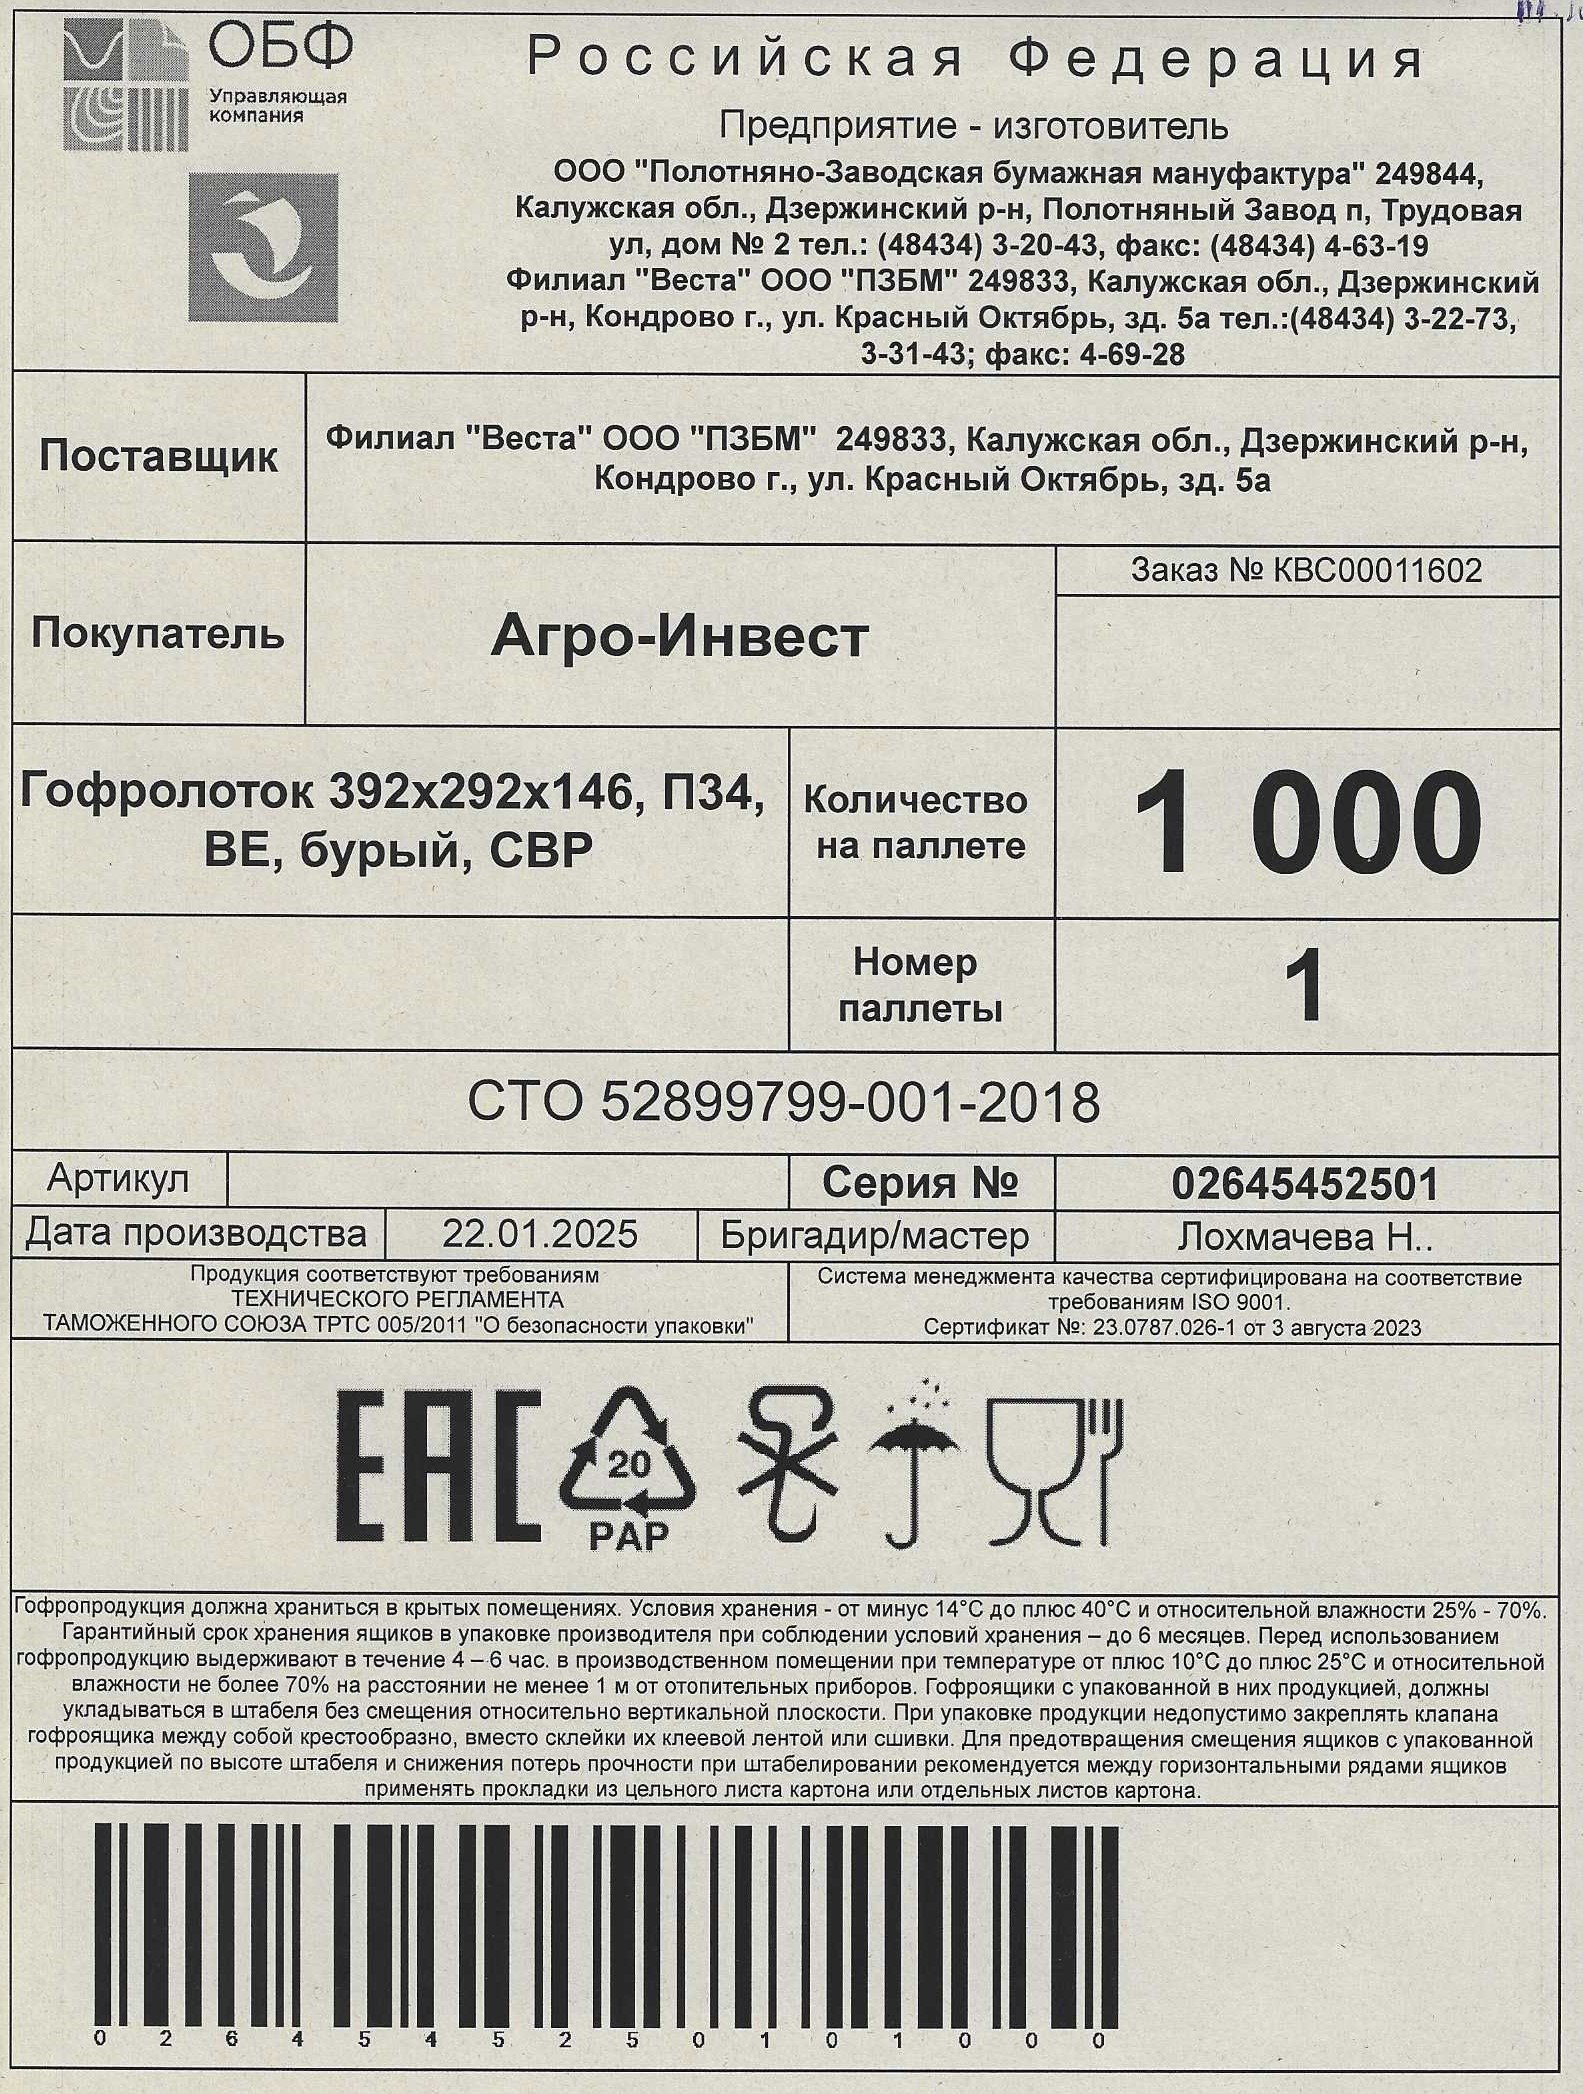
\includegraphics[height=0.9\textheight, keepaspectratio]{Pics/III.10.jpg}
\end{center}
 \caption{Бирки на готовую продукцию}
 \label{pic:III.10}
\end{figure}

\begin{figure}
\begin{center}
 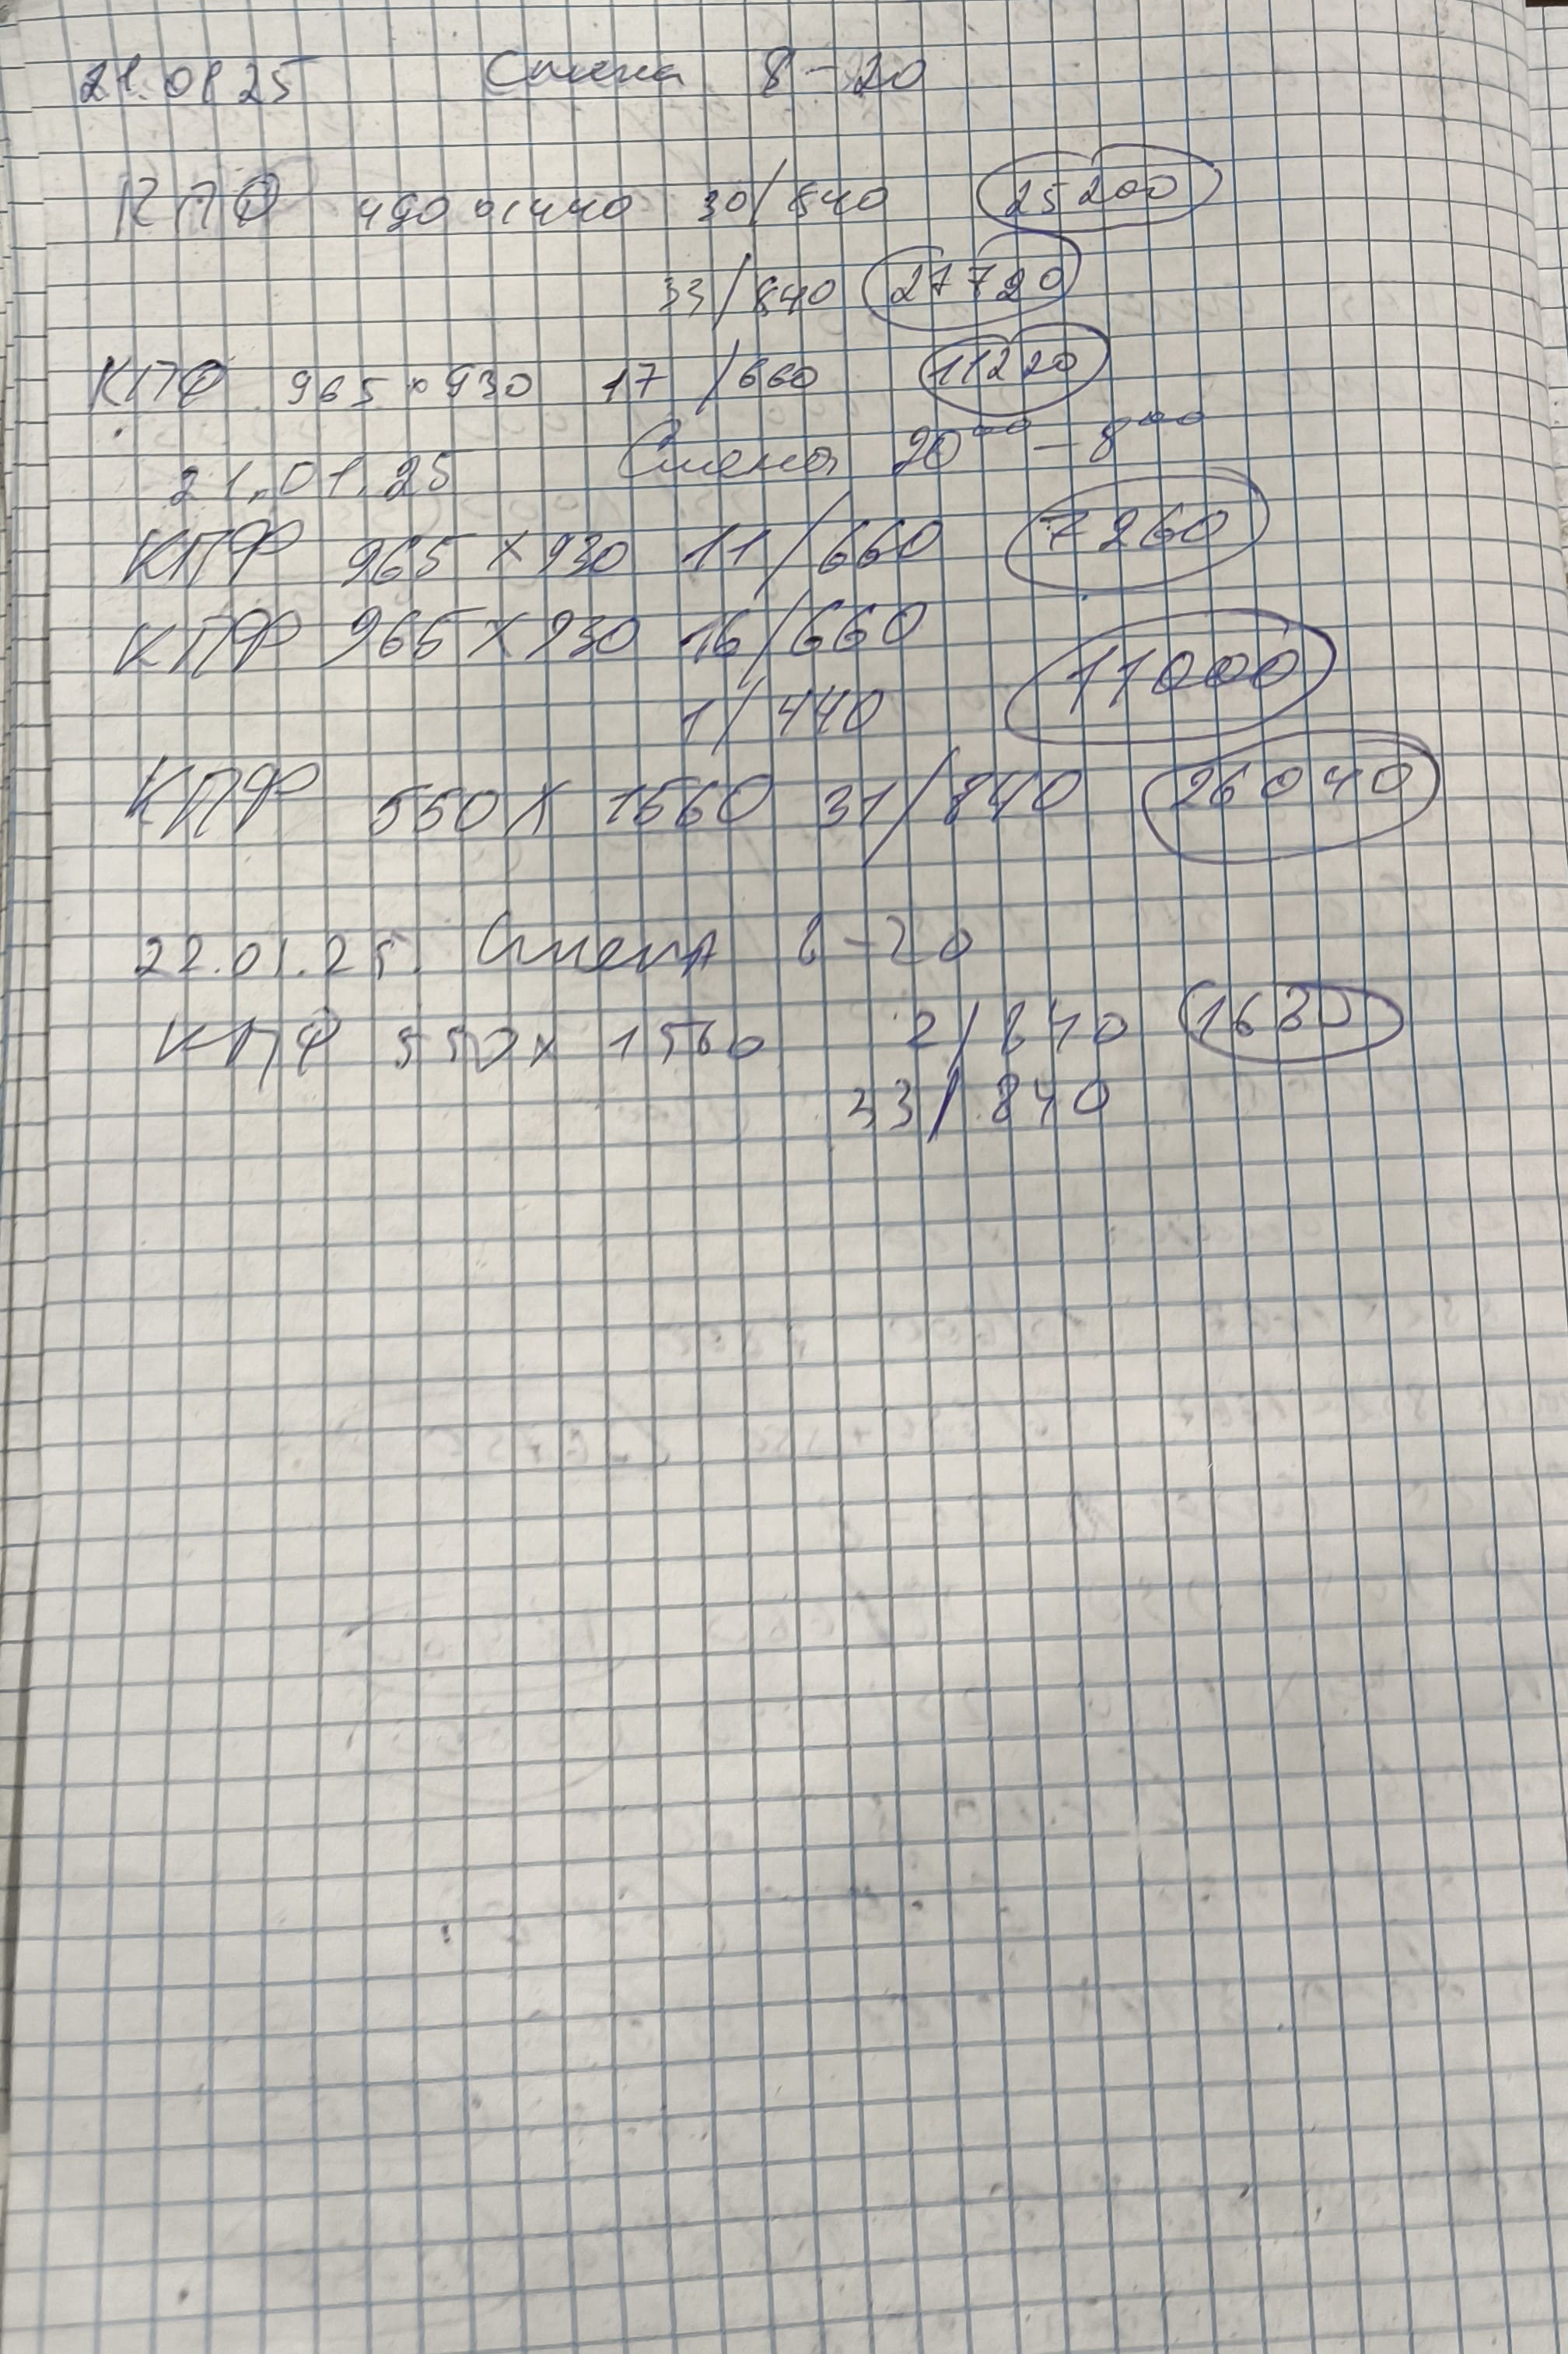
\includegraphics[height=0.9\textheight, keepaspectratio]{Pics/VI журнал машинистов.jpg}
\end{center}
 \caption{Журнал машинистов}
 \label{pic:VI журнал машинистов}
\end{figure}

\begin{figure}
\begin{center}
 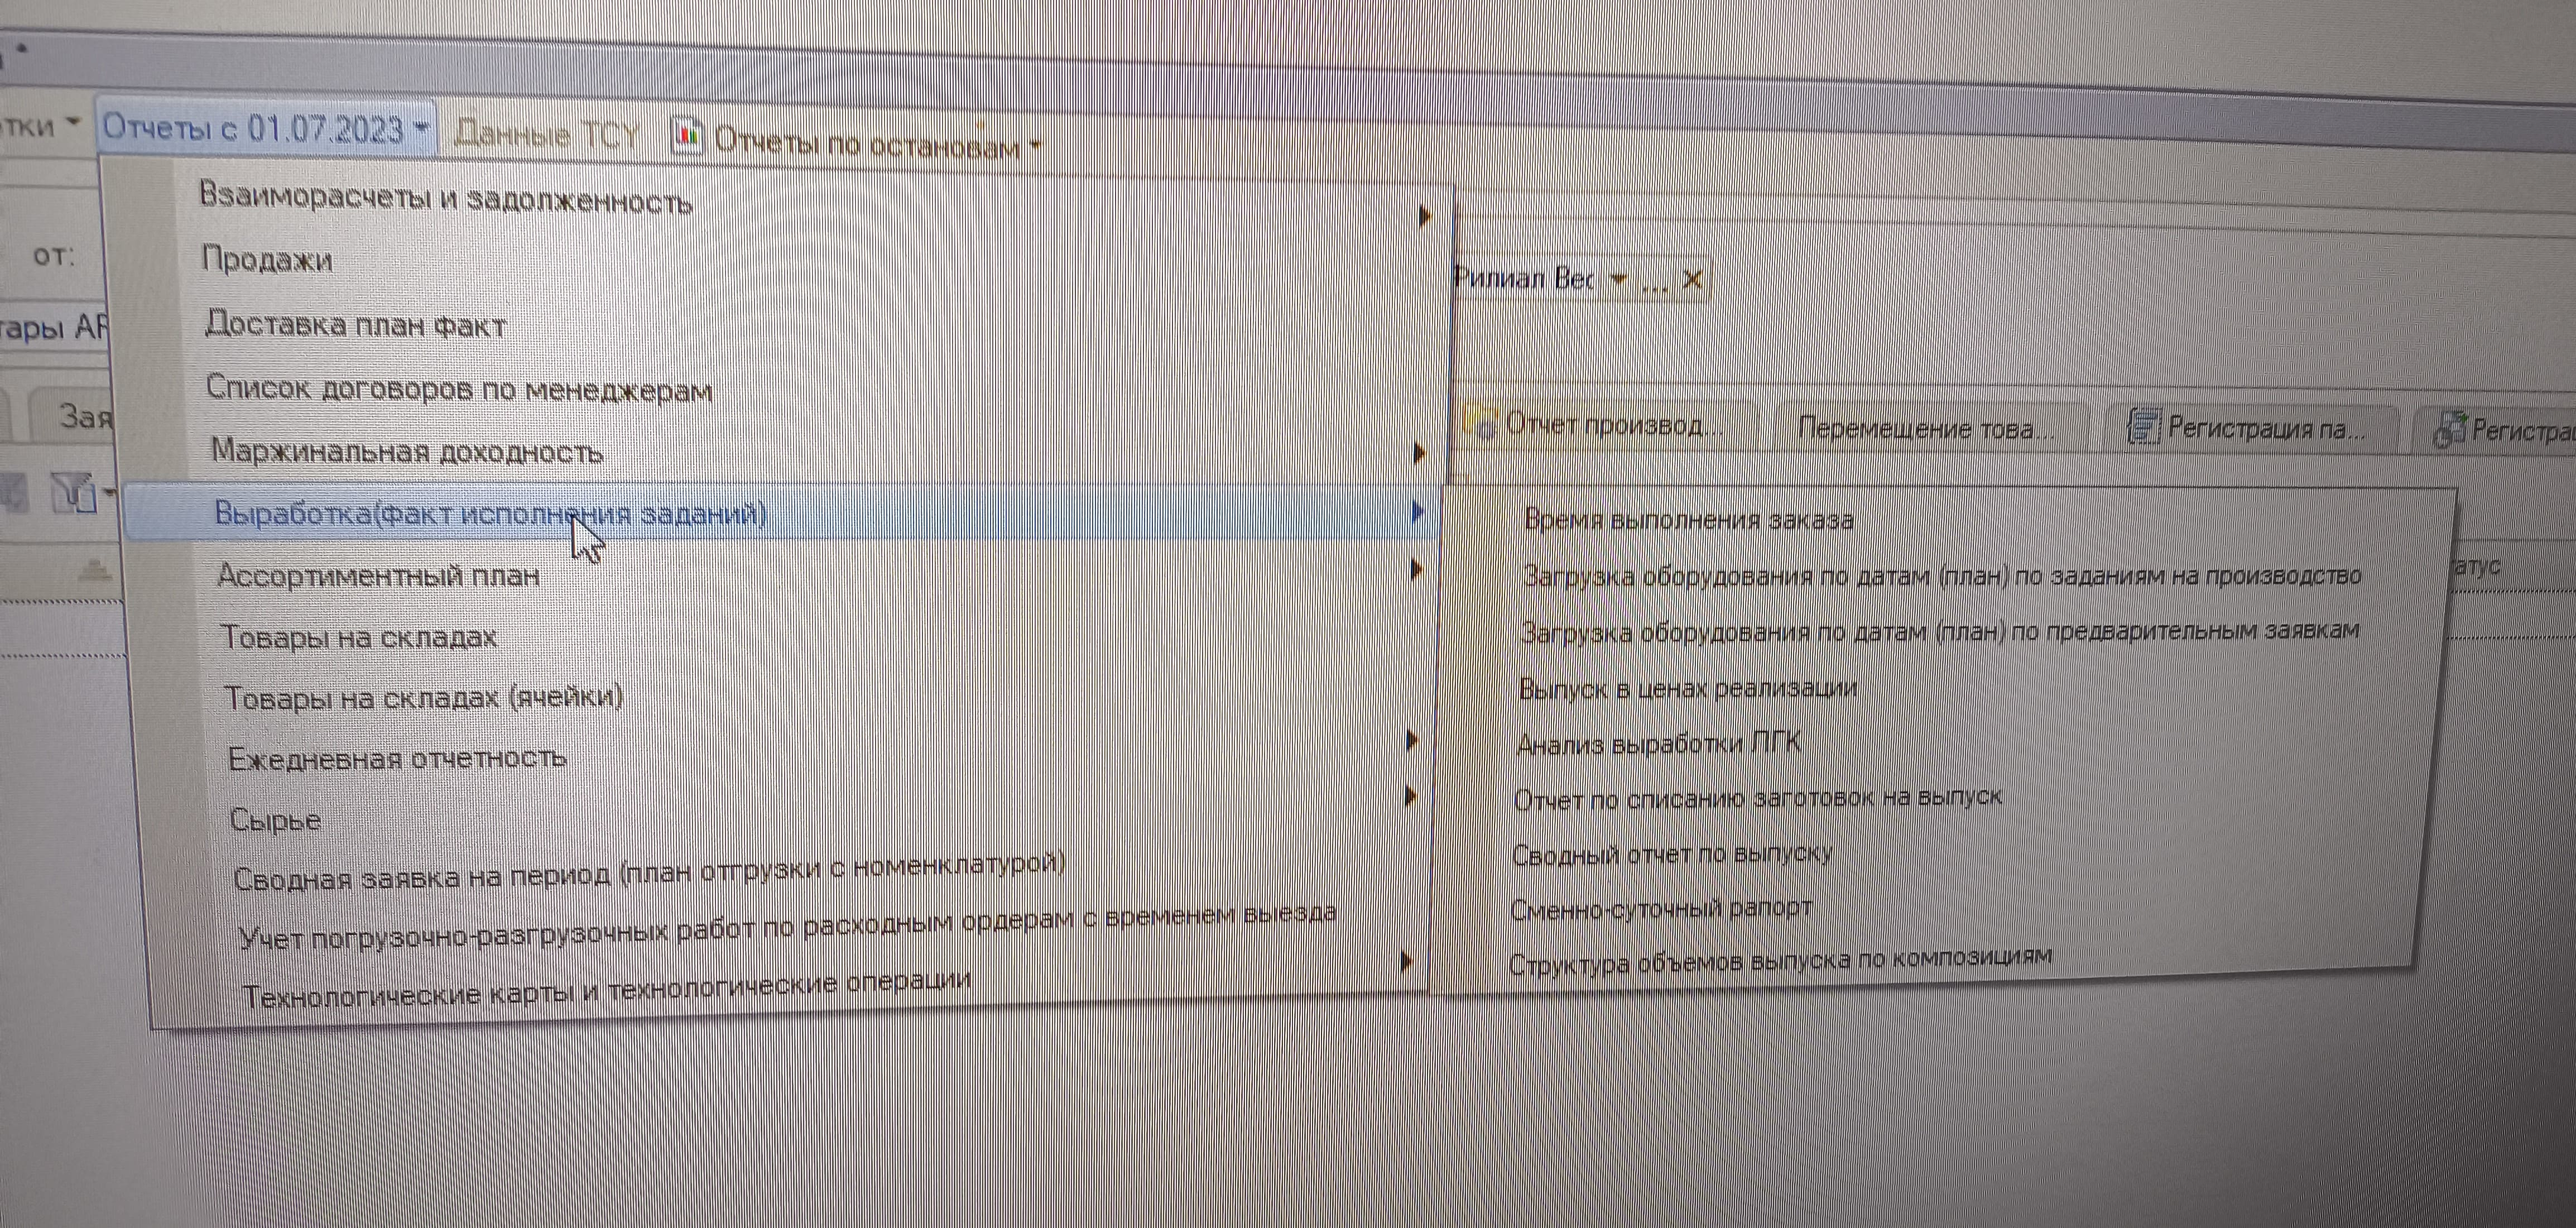
\includegraphics[height=0.32\textheight, keepaspectratio]{Pics/III отчеты 2.jpg}
\end{center}
 \caption{Отчеты в системе 1С: УПП}
 \label{pic:III отчеты 2}
\end{figure}

\begin{figure}
\begin{center}
 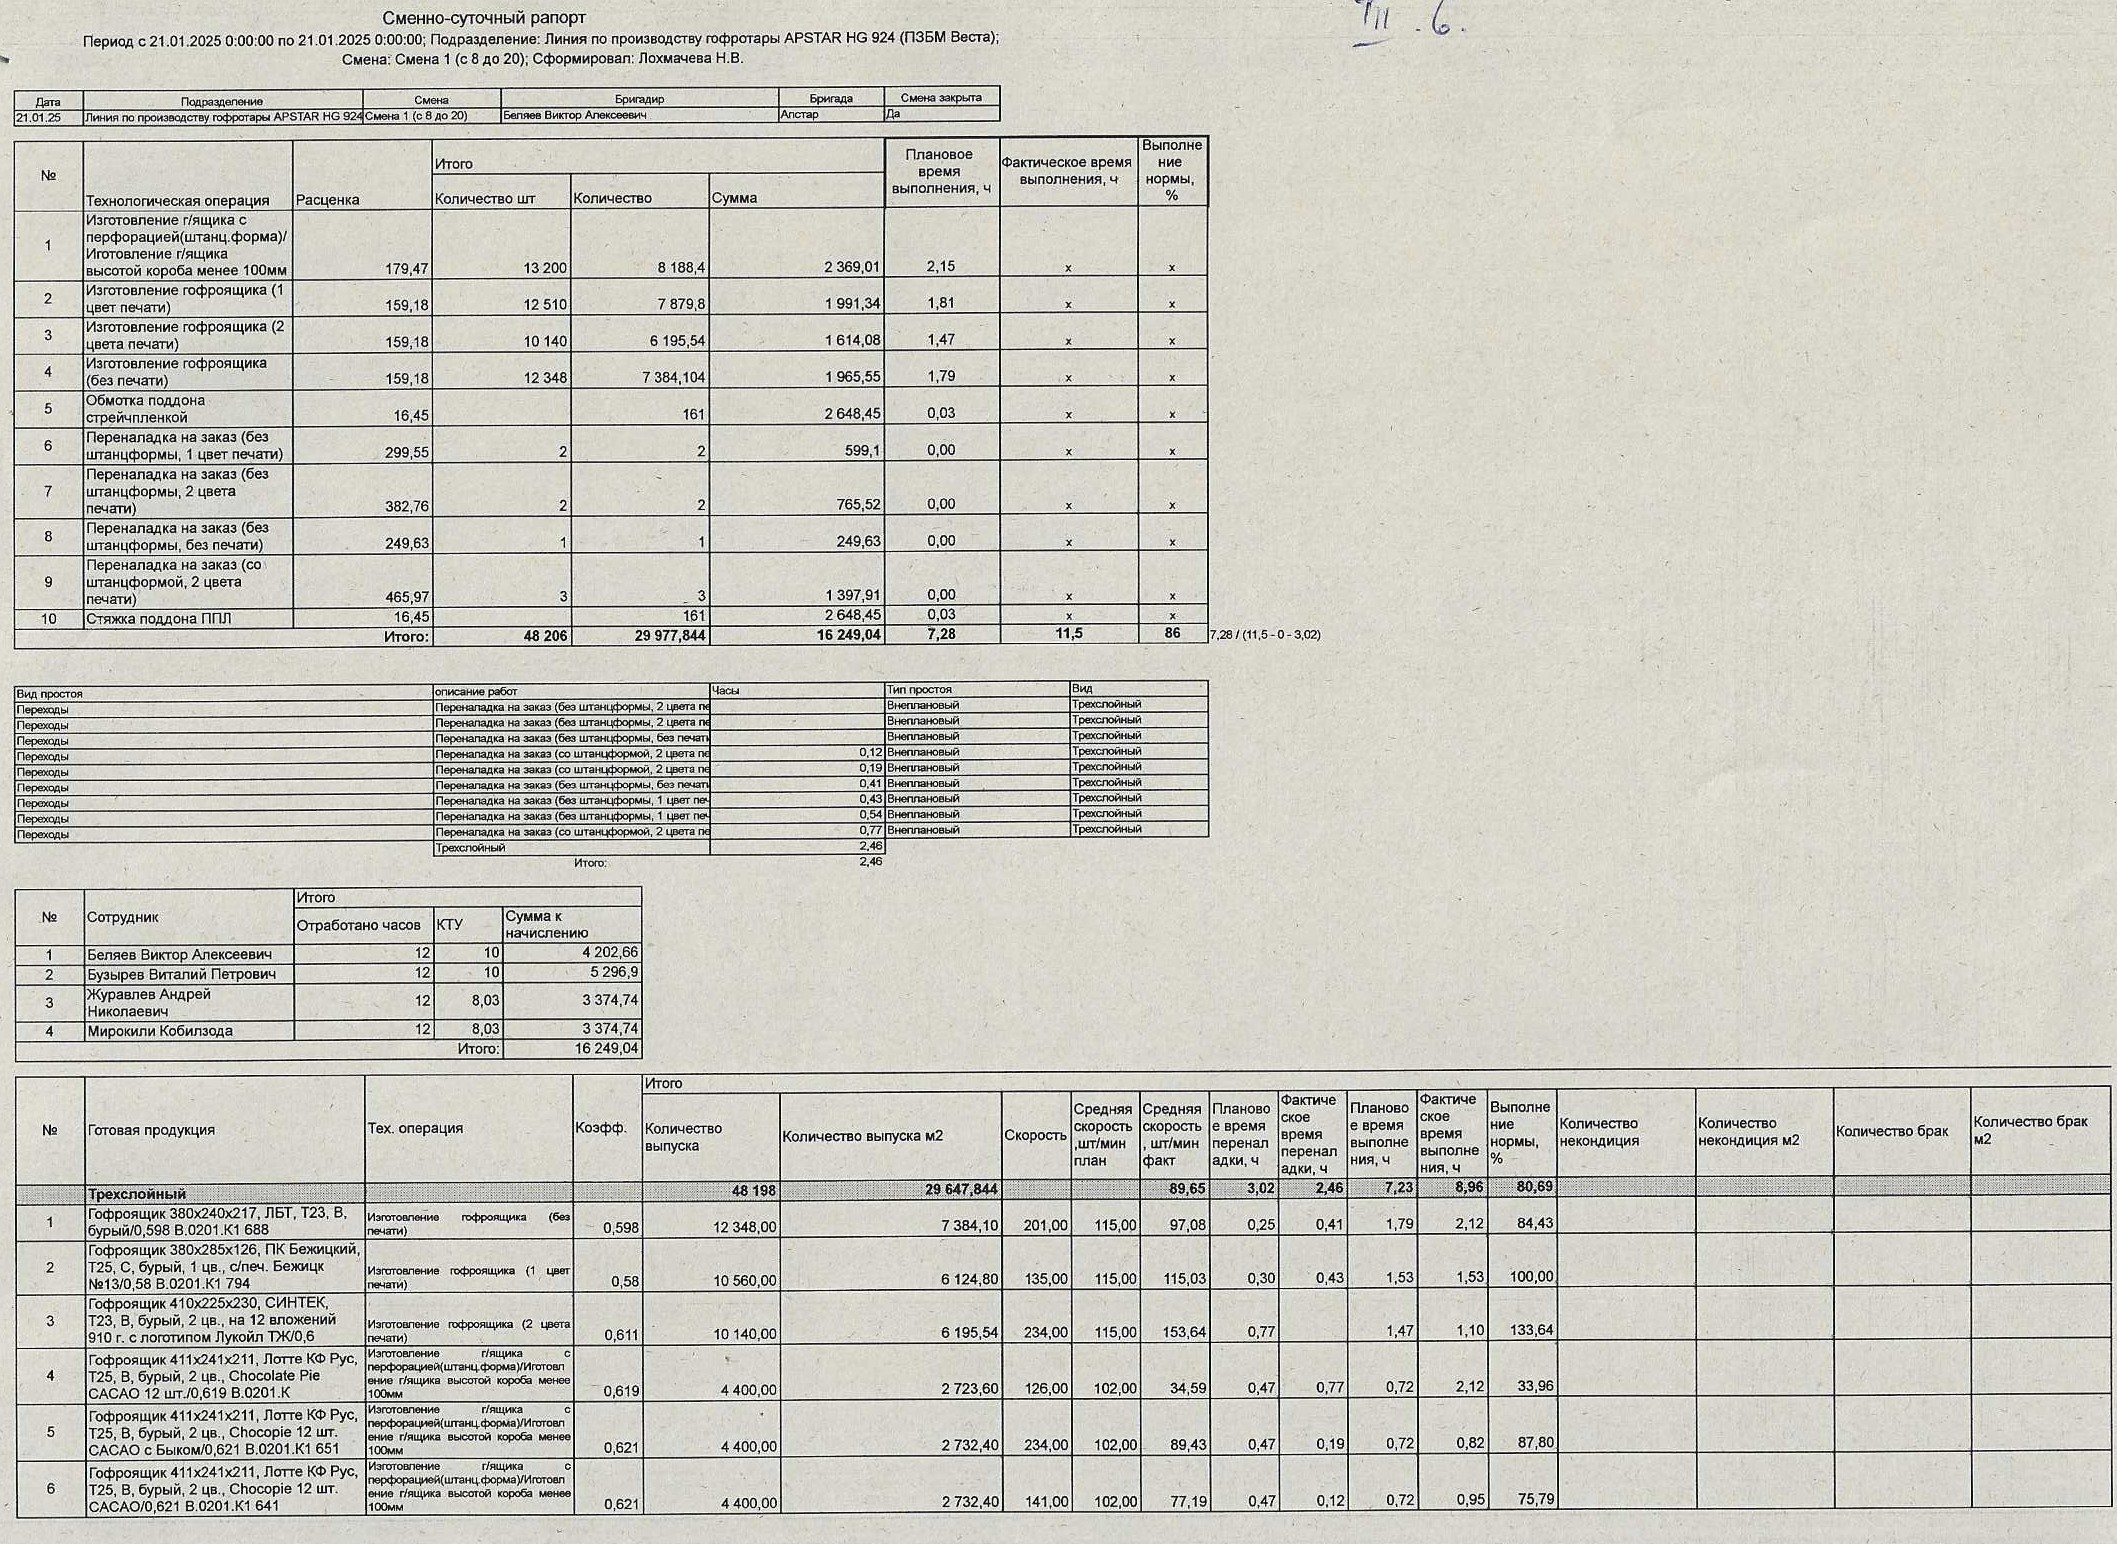
\includegraphics[height=0.5\textheight, keepaspectratio]{Pics/III.6.jpg}
\end{center}
 \caption{Сменно-суточный рапорт}
 \label{pic:III.6}
\end{figure}

\begin{figure}
\begin{center}
 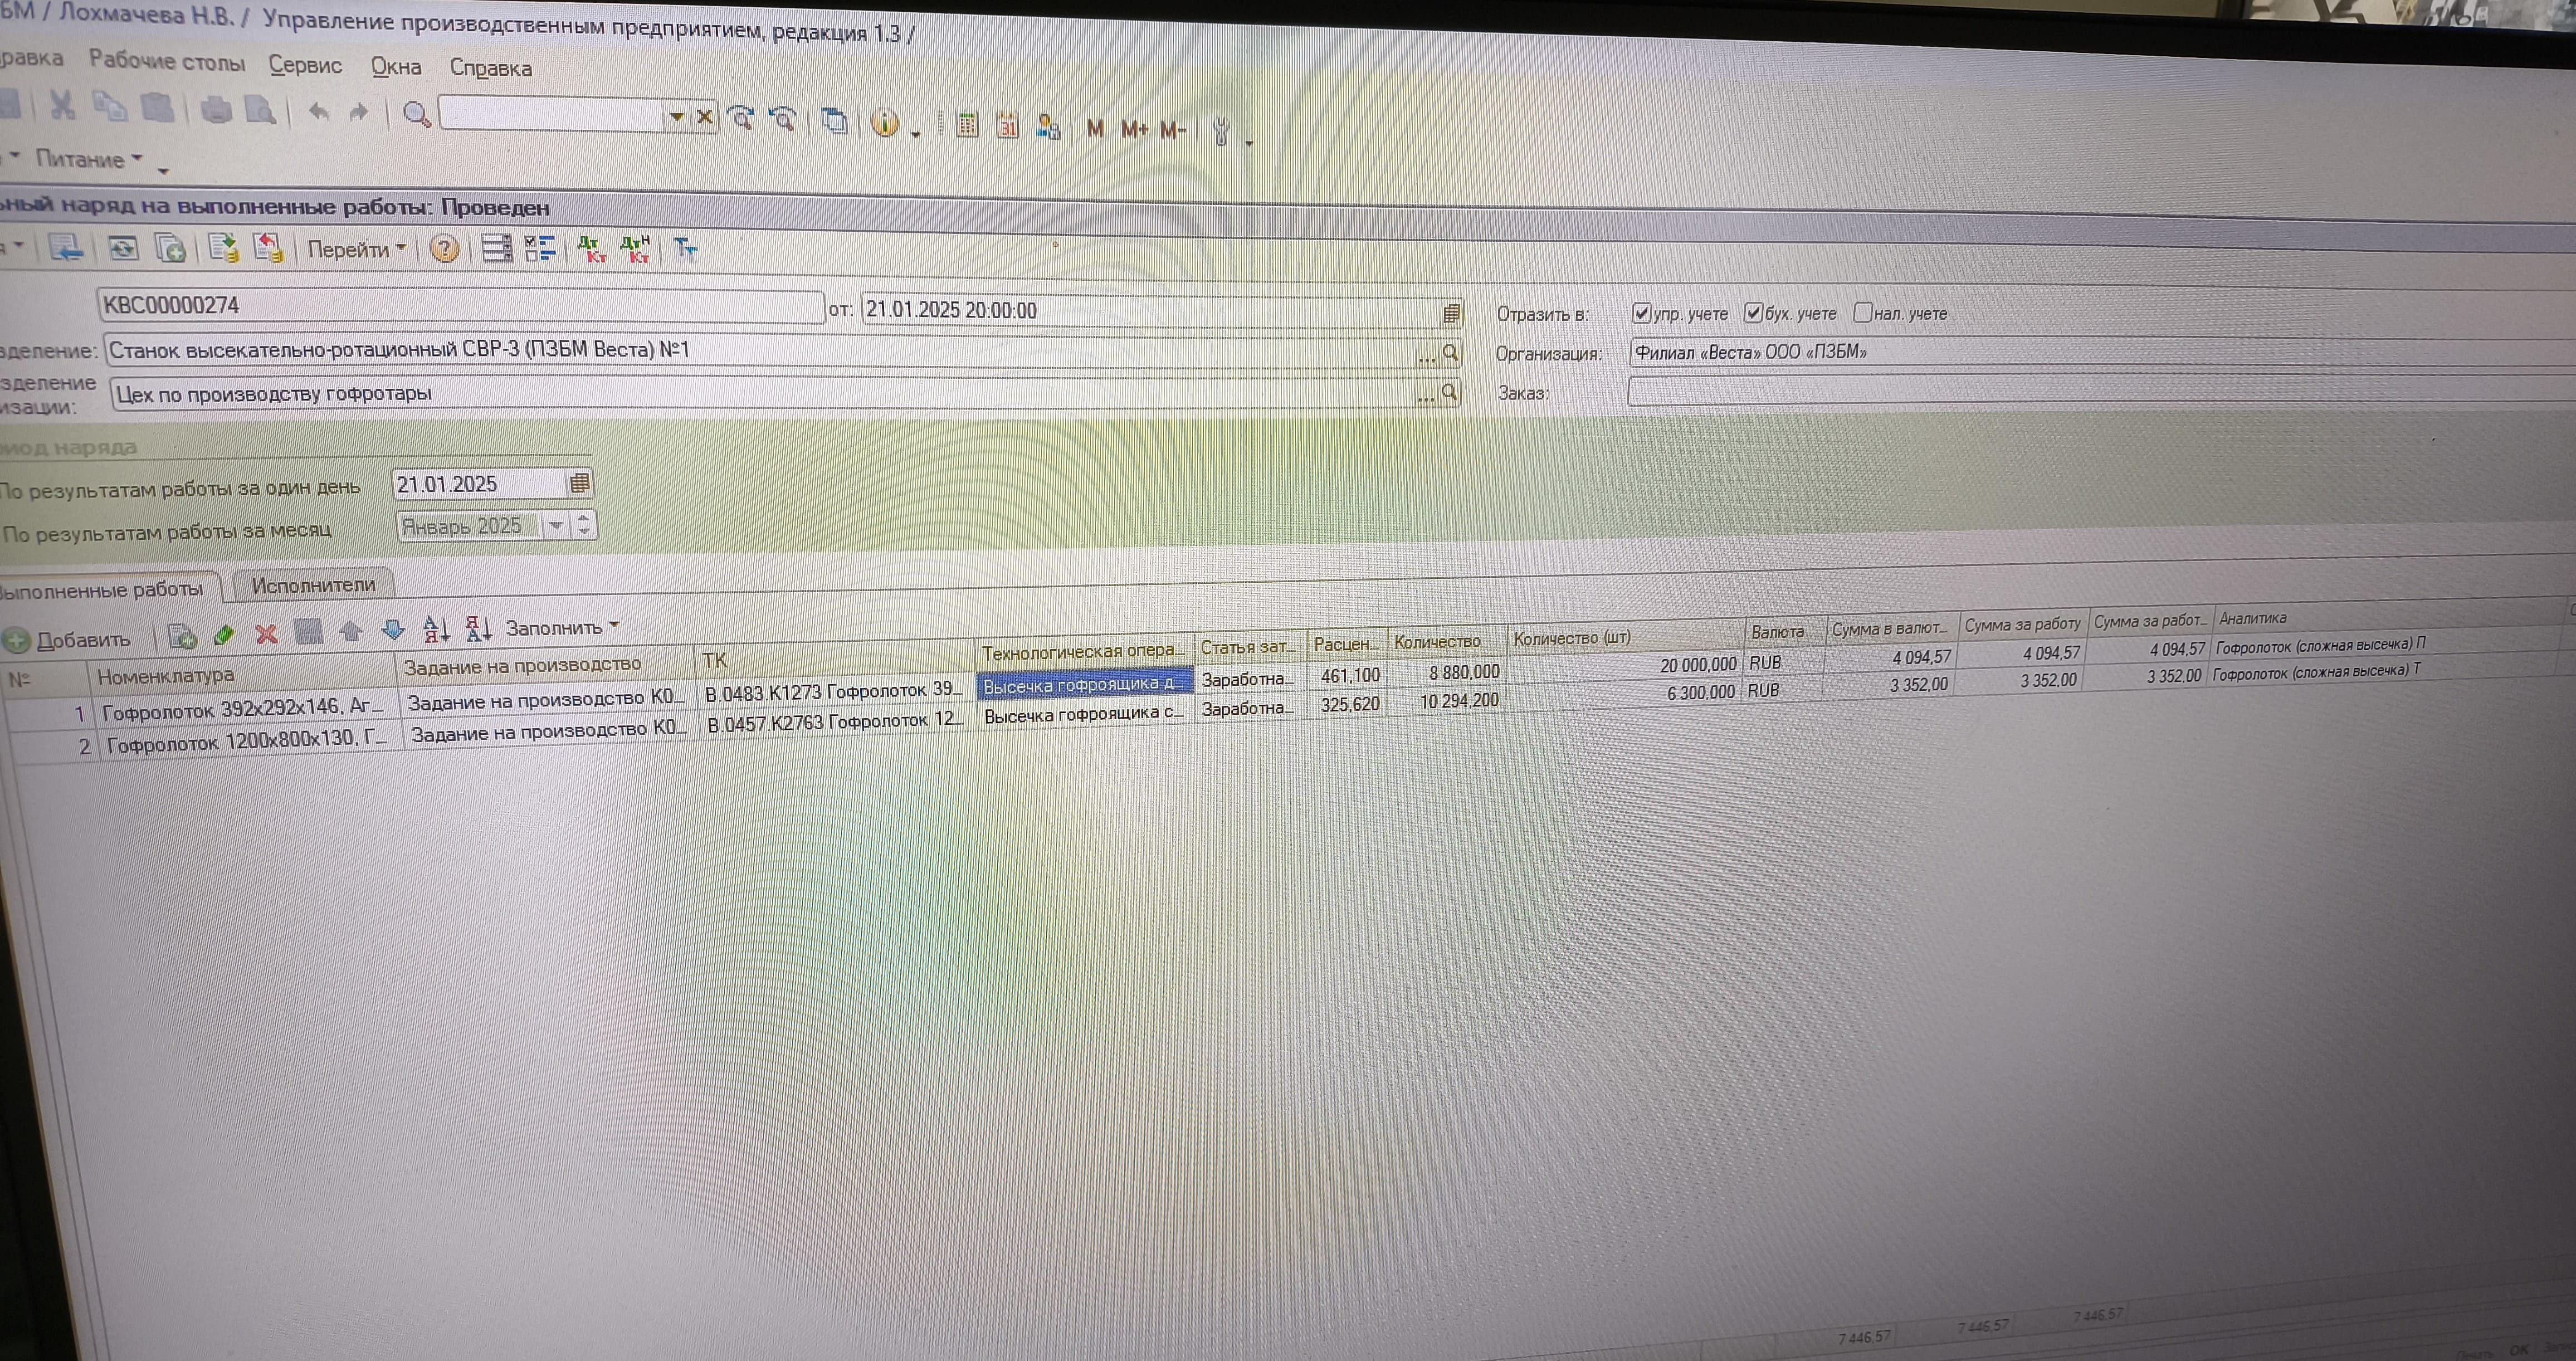
\includegraphics[height=0.35\textheight, keepaspectratio]{Pics/IIIсдельныйнаряд.jpg}
\end{center}
 \caption{Сдельный наряд}
 \label{pic:IIIсдельныйнаряд}
\end{figure}

\begin{figure}
\begin{center}
 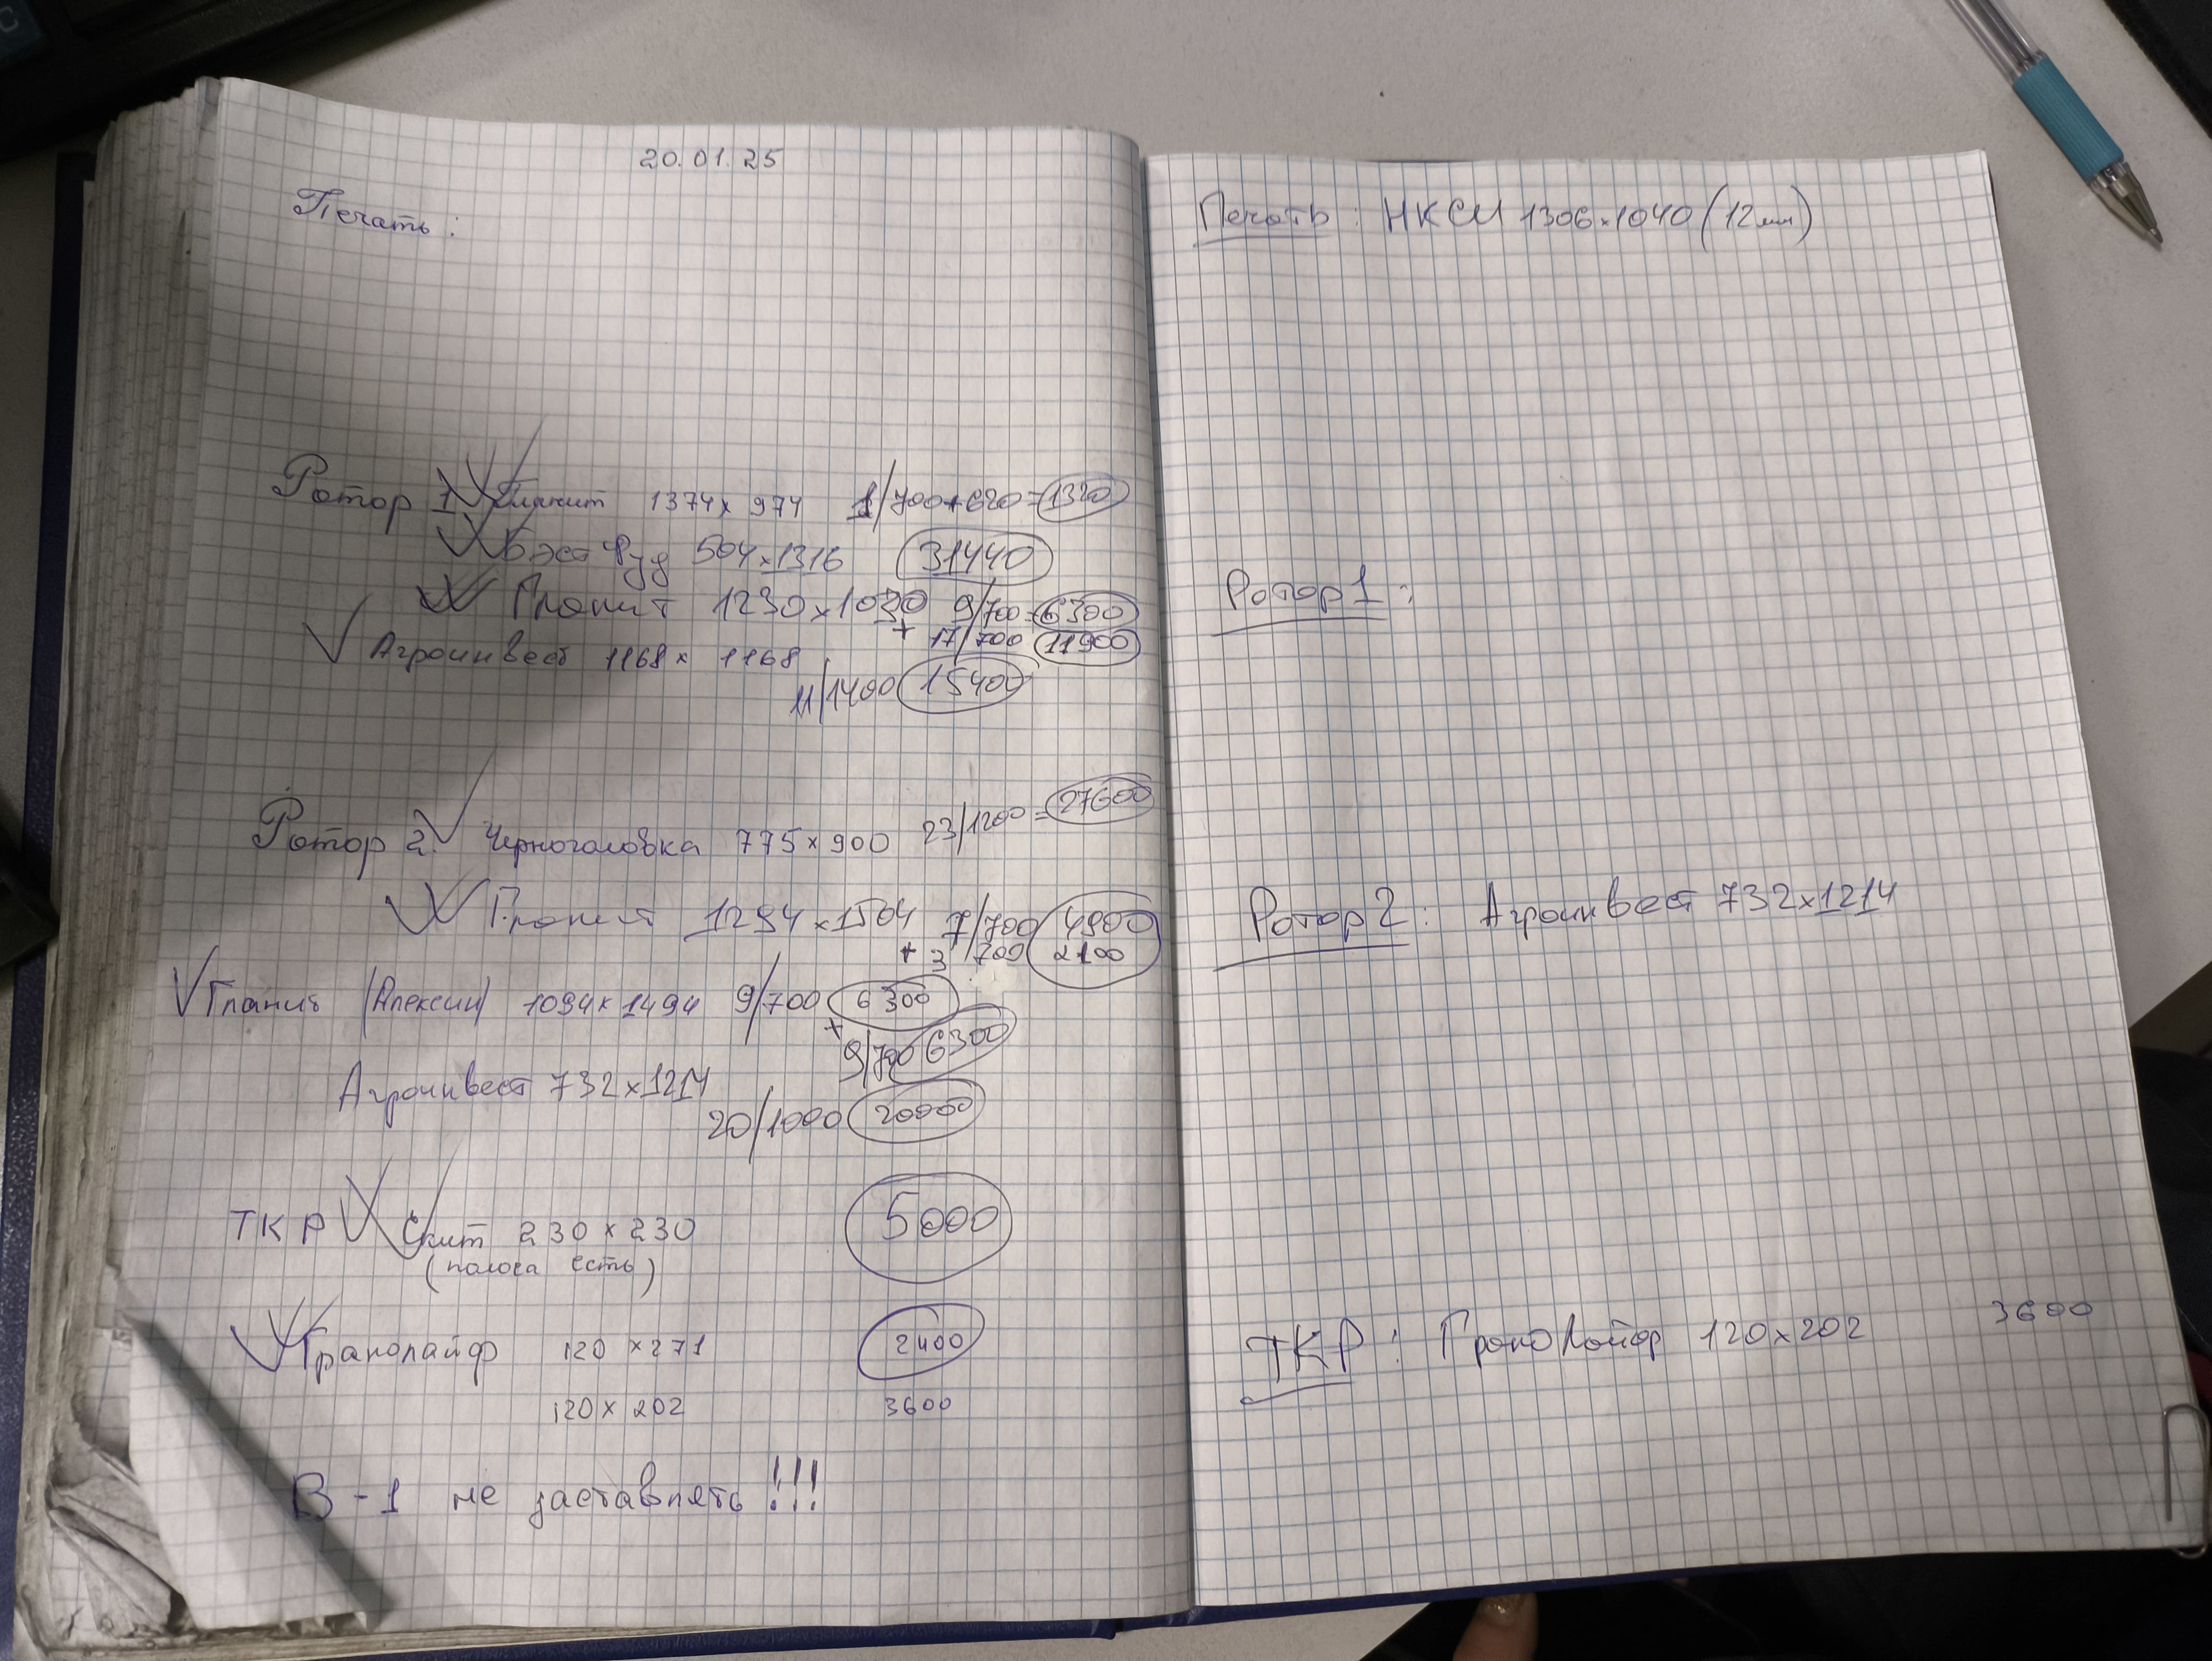
\includegraphics[height=0.5\textheight, keepaspectratio]{Pics/IIIжурналмастера.jpg}
\end{center}
 \caption{Журнал мастеров}
 \label{pic:IIIжурналмастера}
\end{figure}


\clearpage